%implementing document formatting:
\documentclass[a4paper,11pt,fleqn,dvipsnames,oneside,openright,oldfontcommands]{memoir} 	% Openright aabner kapitler paa hoejresider (openany begge)


%%%%%%%%% Indsat random
%makes it possible to refer to the name of a chapter rather than just the number.
\usepackage{nameref}





% ¤¤ Litteraturlisten ¤¤ %
%setting references (using numbers) and supporting i.a. Chicargo-style:
\usepackage{etex}
\usepackage{etoolbox}
\usepackage{keyval}
\usepackage{ifthen}
\usepackage{url}
\usepackage{csquotes}
\usepackage[numbers]{natbib}
%\newcommand{\btx}{Bib\TeX}
%\usepackage[backend=biber,url=true,doi=true,style=numeric, sorting=none]{biblatex}
%\addbibresource{VoresKilder.bib}















%package for writing program code in latex
\usepackage{listings}
%%%%%%%%%%%%%%%%%%%%%%

% ¤¤ Oversaettelse og tegnsaetning ¤¤ %
\usepackage[utf8]{inputenc}					% Input-indkodning af tegnsaet (UTF8)
\usepackage[danish]{babel}					% Dokumentets sprog
\usepackage[T1]{fontenc}					% Output-indkodning af tegnsaet (T1)
\usepackage{ragged2e,anyfontsize}			% Justering af elementer
\usepackage{fixltx2e}						% Retter forskellige fejl i LaTeX-kernen							
								
								
								
																			
% ¤¤ Figurer og tabeller (floats) ¤¤ %
\usepackage{graphicx} 						% Haandtering af eksterne billeder (JPG, PNG, EPS, PDF)
%\usepackage{eso-pic}						% Tilfoej billedekommandoer paa hver side
%\usepackage{wrapfig}						% Indsaettelse af figurer omsvoebt af tekst. \begin{wrapfigure}{Placering}{Stoerrelse}
\usepackage{multirow}                		% Fletning af raekker og kolonner (\multicolumn og \multirow)
\usepackage{multicol}         	        	% Muliggoer output i spalter
\usepackage{rotating}						% Rotation af tekst med \begin{sideways}...\end{sideways}
\usepackage{colortbl} 						% Farver i tabeller (fx \columncolor og \rowcolor)
\usepackage{xcolor}							% Definer farver med \definecolor. Se mere: http://en.wikibooks.org/wiki/LaTeX/Colors
\usepackage{flafter}						% Soerger for at floats ikke optraeder i teksten foer deres reference
\let\newfloat\relax 						% Justering mellem float-pakken og memoir
\usepackage{float}							% Muliggoer eksakt placering af floats, f.eks. \begin{figure}[H]
\usepackage{array,booktabs,xcolor,longtable} % kan lave \hdashline i tabellertabe
\usepackage{arydshln}
\usepackage{tabu}

	
	
% ¤¤ Matematik mm. ¤¤
\usepackage{amsmath , amsfonts , amssymb, float, stmaryrd} 		% Avancerede matematik-udvidelser
%\usepackage{mathtools}						% Andre matematik- og tegnudvidelser
\usepackage{textcomp}                 		% Symbol-udvidelser (f.eks. promille-tegn med \textperthousand )
\usepackage{rsphrase}						% Kemi-pakke til RS-saetninger, f.eks. \rsphrase{R1}
\usepackage[version=3]{mhchem} 				% Kemi-pakke til flot og let notation af formler, f.eks. \ce{Fe2O3}
\usepackage{siunitx}						% Flot og konsistent praesentation af tal og enheder med \si{enhed} og \SI{tal}{enhed}
\sisetup{output-decimal-marker = {,}}		% Opsaetning af \SI (DE for komma som decimalseparator) 

% ¤¤ Referencer og kilder ¤¤ %
\usepackage[danish]{varioref}				% Muliggoer bl.a. krydshenvisninger med sidetal (\vref)
\usepackage[numbers]{natbib}				% Udvidelse med naturvidenskabelige citationsmodeller
%\usepackage{xr}							% Referencer til eksternt dokument med \externaldocument{<NAVN>}
%\usepackage{glossaries}					% Terminologi- eller symbolliste (se mere i Daleifs Latex-bog)
\usepackage{lastpage}					% Gør det mulig at refere til sidste side 

% ¤¤ Misc. ¤¤ %
\usepackage{listings}						% Placer kildekode i dokumentet med \begin{lstlisting}...\end{lstlisting}
\usepackage{lipsum}							% Dummy text \lipsum[..]
\usepackage[shortlabels]{enumitem}			% Muliggoer enkelt konfiguration af lister
\usepackage{pdfpages}						% Goer det muligt at inkludere pdf-dokumenter med kommandoen \includepdf[pages={x-y}]{fil.pdf}	
\pdfoptionpdfminorversion=6					% Muliggoer inkludering af pdf dokumenter, af version 1.6 og hoejere
\pretolerance=2500 							% Justering af afstand mellem ord (hoejt tal, mindre orddeling og mere luft mellem ord)


% Kommentarer og rettelser med \fxnote. Med 'final' i stedet for 'draft' udloeser hver note en error i den faerdige rapport.
\usepackage[footnote,draft,danish,silent,nomargin]{fixme}		


%%%% CUSTOM SETTINGS %%%%

% ¤¤ Marginer ¤¤ %
\setlrmarginsandblock{3.5cm}{2.5cm}{*}		% \setlrmarginsandblock{Indbinding}{Kant}{Ratio}
\setulmarginsandblock{2.5cm}{3.0cm}{*}		% \setulmarginsandblock{Top}{Bund}{Ratio}
\checkandfixthelayout 						% Oversaetter vaerdier til brug for andre pakker

%	¤¤ Afsnitsformatering ¤¤ %
\setlength{\parindent}{6mm}           		% Stoerrelse af indryk
\setlength{\parskip}{0mm}          			% Afstand mellem afsnit ved brug af double Enter
\linespread{1,1}							% Linie afstand



% ¤¤ Indholdsfortegnelse ¤¤ %
\setsecnumdepth{subsection}		 			% Dybden af nummerede overkrifter (part/chapter/section/subsection)
\maxsecnumdepth{subsection}					% Dokumentklassens graense for nummereringsdybde
\settocdepth{subsection} 					% Dybden af indholdsfortegnelsen

% ¤¤ Lister ¤¤ %
\setlist{
  topsep=0pt,								% Vertikal afstand mellem tekst og listen
  itemsep=-1ex,								% Vertikal afstand mellem items
} 

%hyperlinks in the tabel of contents - comment this out before the report is printed.
\usepackage{hyperref}
\hypersetup{
	bookmarks = true,  % Show 'bookmark'-frame in pdf.
	colorlinks = true, % True = colored links, False = framed links.
	citecolor = black,  % Link color for references.
	linkcolor = black,  % Link color in table of contents.
	urlcolor = black,   % Link color for extern URLs.
}

% ¤¤ Opsaetning af figur- og tabeltekst ¤¤ %
\usepackage{caption}
\usepackage{subcaption}
\captionnamefont{\small\bfseries\itshape}	% Opsaetning af tekstdelen ('Figur' eller 'Tabel')
\captiontitlefont{\small}					% Opsaetning af nummerering
\captiondelim{. }							% Seperator mellem nummerering og figurtekst
\hangcaption								% Venstrejusterer flere-liniers figurtekst under hinanden
%\captionwidth{0.9\textwidth}					% Bredden af figurteksten
\setlength{\belowcaptionskip}{0pt}			% Afstand under figurteksten
\captionsetup[figure]{labelfont={bf,it},font={it}} % sætter nummer til fed og kursis. Resten til fed + skriften er mindre end resten
\captionsetup[table]{labelfont={bf,it},font={it}} 


% ¤¤ Opsaetning af listings ¤¤ %

\definecolor{commentGreen}{RGB}{34,139,24}
\definecolor{stringPurple}{RGB}{208,76,239}

\lstset{language=Matlab,					% Sprog
	basicstyle=\ttfamily\scriptsize,		% Opsaetning af teksten
	keywords={for,if,while,else,elseif,		% Noegleord at fremhaeve
			  end,break,return,case,
			  switch,function},
	keywordstyle=\color{blue},				% Opsaetning af noegleord
	commentstyle=\color{commentGreen},		% Opsaetning af kommentarer
	stringstyle=\color{stringPurple},		% Opsaetning af strenge
	showstringspaces=false,					% Mellemrum i strenge enten vist eller blanke
	numbers=left, numberstyle=\tiny,		% Linjenumre
	extendedchars=true, 					% Tillader specielle karakterer
	columns=flexible,						% Kolonnejustering
	breaklines, breakatwhitespace=true,		% Bryd lange linjer
}

% ¤¤ Navngivning ¤¤ %
\addto\captionsdanish{
	\renewcommand\appendixname{Bilag}
	\renewcommand\contentsname{Indholdsfortegnelse}	
	\renewcommand\appendixpagename{Bilag}
	\renewcommand\appendixtocname{Bilag}
	\renewcommand\cftchaptername{\chaptername~}				% Skriver "Kapitel" foran kapitlerne i indholdsfortegnelsen
	\renewcommand\cftappendixname{\appendixname~}			% Skriver "Appendiks" foran appendiks i indholdsfortegnelsen
}

% ¤¤ Kapiteludssende ¤¤ %
%\definecolor{numbercolor}{gray}{0.7}		% Definerer en farve til brug til kapiteludseende
%\newif\ifchapternonum

\makechapterstyle{AAU}
{
	% Afstand mellem sidehovedet og kapitel+tal+kapitelnavnet defineres til:
	\setlength{\beforechapskip}{0cm}

	% Afstanden mellem kapitelnavnet og body-teksten defineres til:
	\setlength{\afterchapskip}{2cm}

	% Typografiopsætningen til kapitel+tal defineres til:
	\renewcommand\chapnamefont{\sffamily\bfseries\LARGE\raggedright}
	
	% Typografiopsætningen til kapitel+tal defineres til:
	\renewcommand\chaptitlefont{\sffamily\bfseries\huge\color[cmyk]{1.00,0.38,0.00,0.64}}

	% Forårsager, at der til kapitlet også tilføjes dets respektive tal:
	\renewcommand\chapternamenum{}
	\renewcommand\printchapternum
	{
		\makebox[0pt][l]
		{
			\color[cmyk]{1.00,0.38,0.00,0.64}
			\hspace{0.1cm}
			\resizebox{!}{1cm}{\chapnamefont\bfseries\sffamily\thechapter}
		}
	}
	
	% Definitionen af linjenstykket mellem ``Kapitel #'' samt ``kapitelnavnet'':
			\renewcommand\afterchaptertitle{\par\hspace{1.5cm}\hrule height 1pt\vskip\midchapskip}
}

% Aktivering af selve kapitellayoutet med dét navn, som definerer kapitellayoutet (ses fra tidligere):
\chapterstyle{AAU}

%\makechapterstyle{jenor}{					% Definerer kapiteludseende frem til ...
%  \renewcommand\beforechapskip{0pt}
%  \renewcommand\printchaptername{}
%  \renewcommand\printchapternum{}
% % \renewcommand\printchapternonum{\chapternonumtrue}
%  \renewcommand\chaptitlefont{\fontfamily{pbk}\fontseries{db}\fontshape{n}\fontsize{20}{25}\selectfont\raggedright}
%  \renewcommand\chapnumfont{\fontfamily{pbk}\fontseries{m}\fontshape{n}\fontsize{1in}{0in}\selectfont\color{numbercolor}}
% \renewcommand\printchaptertitle[1]{
%    \noindent
%    \ifchapternum
%     \begin{tabularx}{\textwidth}{XI}
%	{\let\\\newline\chaptitlefont ##1\par}     
%    \end{tabularx}
%    \par\vskip-2.5mm\hrule
%    \else
%    \begin{tabularx}{\textwidth}{X}
%      {\parbox[b]{\linewidth}{\chaptitlefont ##1}} & \raisebox{-15pt}{\chapnumfont \thechapter}
%    \end{tabularx}
%    \par\vskip2mm\hrule
%    \fi
%  }
%}											% ... her
%
%\chapterstyle{jenor}						% Valg af kapiteludseende - Google 'memoir chapter styles' for alternativer

% ¤¤ Sidehoved ¤¤ %

\makepagestyle{AAU}							% Definerer sidehoved og sidefod udseende frem til ...
\makepsmarks{AAU}{%
	\createmark{chapter}{left}{shownumber}{}{. \ }
	\createmark{section}{right}{shownumber}{}{. \ }
	\createplainmark{toc}{both}{\contentsname}
	\createplainmark{lof}{both}{\listfigurename}
	\createplainmark{lot}{both}{\listtablename}
	%\createplainmark{bib}{both}{\bibname}
	\createplainmark{index}{both}{\indexname}
	\createplainmark{glossary}{both}{\glossaryname}
}
\nouppercaseheads											% Ingen Caps oenskes

\makeoddhead{AAU}{Gruppe B206}{}{\leftmark}				% Definerer lige siders sidehoved (\makeevenhead{Navn}{Venstre}{Center}{Hoejre})
\makeevenhead{AAU}{\rightmark}{}{Aalborg Universitet}		% Definerer ulige siders sidehoved (\makeoddhead{Navn}{Venstre}{Center}{Hoejre})
\makeevenfoot{AAU}{\thepage\ af \pageref{LastPage}}{}{}							% Definerer lige siders sidefod (\makeevenfoot{Navn}{Venstre}{Center}{Hoejre})
\makeoddfoot{AAU}{}{}{\thepage\ af \pageref{LastPage}}								% Definerer ulige siders sidefod (\makeoddfoot{Navn}{Venstre}{Center}{Hoejre})
\makeheadrule{AAU}{\textwidth}{0.5pt}						% Tilfoejer en streg under sidehovedets indhold
\makefootrule{AAU}{\textwidth}{0.5pt}{1mm}					% Tilfoejer en streg under sidefodens indhold

\copypagestyle{AAUchap}{AAU}								% Sidehoved for kapitelsider defineres som standardsider, men med blank sidehoved
\makeoddhead{AAUchap}{}{}{}
\makeevenhead{AAUchap}{}{}{}
\makeheadrule{AAUchap}{\textwidth}{0pt}
\aliaspagestyle{chapter}{AAUchap}							% Den ny style vaelges til at gaelde for chapters
															% ... her
															
\pagestyle{AAU}												% Valg af sidehoved og sidefod


%%%% CUSTOM COMMANDS %%%%

% ¤¤ Billede hack ¤¤ %
\newcommand{\figur}[4]{
		\begin{figure}[H] \centering
			\includegraphics[width=#1\textwidth]{billeder/#2}
			\caption{#3}\label{#4}
		\end{figure} 
}

% ¤¤ Specielle tegn ¤¤ %
\newcommand{\decC}{^{\circ}\text{C}}
\newcommand{\dec}{^{\circ}}
\newcommand{\m}{\cdot}


%%%% ORDDELING %%%%

\hyphenation{}

%%%%Fra engelsk til dansk i \autoref{•} %%%%
\renewcommand{\figureautorefname}{Figur}
\renewcommand{\sectionautorefname}{Afsnit}
\renewcommand{\subsectionautorefname}{Afsnit}
\renewcommand{\subsubsectionautorefname}{Afsnit}
\renewcommand{\tableautorefname}{Tabel}
\renewcommand{\appendixautorefname}{Bilag}
\renewcommand{\equationautorefname}{Ligning}
\renewcommand{\itemautorefname}{Punkt}
\renewcommand{\chapterautorefname}{Kapitel}
%Figure references:
\newcommand{\figref}[1]{\textbf{figure \ref{#1}}}

%Figure references after full stop/period:
\newcommand{\Figref}[1]{\textbf{Figure \ref{#1}}}

%Table references:
\newcommand{\tableref}[1]{\textbf{table \ref{#1}}}

%Table references after full stop/period:
\newcommand{\Tableref}[1]{\textbf{Table \ref{#1}}}

%Units:
%inserting '\omit' before '{\put' prior ot final compile will fix allignment (and generate errors)
\newcommand{\unit}[1]{{\put(300,0){$\hfill\left[\: #1 \:\right]$}}}

%Text:
\newcommand{\tx}[1]{\text{#1}}

%Equation references:
%1 equation:
\renewcommand{\eqref}[1]{\textbf{equation (\ref{#1})}}
%2 equations:
\newcommand{\eqrefTwo}[2]{\textbf{equation (\ref{#1})} and \textbf{(\ref{#2})}}
%3 equations:
\newcommand{\eqrefThree}[3]{\textbf{equation (\ref{#1})}, \textbf{(\ref{#2})} and \textbf{(\ref{#3})}}
%4 equations:
\newcommand{\eqrefFour}[4]{\textbf{equation (\ref{#1})}, \textbf{(\ref{#2})}, \textbf{(\ref{#3})} and \textbf{(\ref{#4})}}
%5 equations:
\newcommand{\eqrefFive}[5]{\textbf{equation (\ref{#1})}, \textbf{(\ref{#2})}, \textbf{(\ref{#3})}, \textbf{(\ref{#4})} and \textbf{(\ref{#5})}}
%5 equations:
\newcommand{\eqrefSix}[6]{\textbf{equation (\ref{#1})}, \textbf{(\ref{#2})}, \textbf{(\ref{#3})}, \textbf{(\ref{#4})}, \textbf{(\ref{#5})} and \textbf{(\ref{#6})}}
%5 equations:
\newcommand{\eqrefSeven}[7]{\textbf{equation (\ref{#1})}, \textbf{(\ref{#2})}, \textbf{(\ref{#3})}, \textbf{(\ref{#4})}, \textbf{(\ref{#5})}, \textbf{(\ref{#6})} and \textbf{(\ref{#7})}}

%Equation references after full stop/period:
%1 equation:
\newcommand{\Eqref}[1]{\textbf{Equation (\ref{#1})}}
%2 equations:
\newcommand{\EqrefTwo}[2]{\textbf{Equation (\ref{#1})} and \textbf{(\ref{#2})}}
%3 equations:
\newcommand{\EqrefThree}[3]{\textbf{Equation (\ref{#1})}, \textbf{(\ref{#2})} and \textbf{(\ref{#3})}}
%4 equations:
\newcommand{\EqrefFour}[4]{\textbf{Equation (\ref{#1})}, \textbf{(\ref{#2})}, \textbf{(\ref{#3})} and \textbf{(\ref{#4})}}
%5 equations:
\newcommand{\EqrefFive}[5]{\textbf{Equation (\ref{#1})}, \textbf{(\ref{#2})}, \textbf{(\ref{#3})}, \textbf{(\ref{#4})} and \textbf{(\ref{#5})}}
%5 equations:
\newcommand{\EqrefSix}[6]{\textbf{Equation (\ref{#1})}, \textbf{(\ref{#2})}, \textbf{(\ref{#3})}, \textbf{(\ref{#4})}, \textbf{(\ref{#5})} and \textbf{(\ref{#6})}}
%5 equations:
\newcommand{\EqrefSeven}[7]{\textbf{Equation (\ref{#1})}, \textbf{(\ref{#2})}, \textbf{(\ref{#3})}, \textbf{(\ref{#4})}, \textbf{(\ref{#5})}, \textbf{(\ref{#6})} and \textbf{(\ref{#7})}}
\begin{document}

%---------------------------INPUTS-------------------------------
%numbers the pages with Roman numeral - starts from "i":
\frontmatter

\clearpage
\thispagestyle{empty}

%\begin{figure}[H]
%	\raggedleft
%		
\includegraphics[width=0.2\textwidth]{figures/aaulogo-da.png}
%\end{figure}


%\vspace*{\fill} 
%\begin{center}	
%	\begin{Huge}
%		P3 Projektrapport - efterår 2015\\
%		\vspace{5 mm}
%		\textbf{System til detektering af kropsbalance}\\
%		\vspace{3 mm}
%		Gruppe 375
%	\end{Huge}
%\end{center}
%\vspace*{\fill}

\begin{center}
\vspace*{\baselineskip}
\rule{\textwidth}{1.6pt}\vspace*{-\baselineskip}\vspace*{2pt} % Thick horizontal line
\rule{\textwidth}{0.4pt}\\[\baselineskip] % Thin horizontal line

{\LARGE System til detektering af kropsbalance\\[0.3\baselineskip] \large P3 Projektrapport}\\[0.2\baselineskip] % Title

\rule{\textwidth}{0.4pt}\vspace*{-\baselineskip}\vspace{3.2pt} % Thin horizontal line
\rule{\textwidth}{1.6pt}\\[\baselineskip] % Thick horizontal line

\vspace*{3\baselineskip}

\scshape % Small caps
Aalborg universitet,  02/09/15-16/12/15 \par % Location and year

\vspace*{2\baselineskip} % Whitespace between location/year and editors

Skrevet af \\[\baselineskip]
{\Large Gruppe B203\par}
\end{center} % Center all text

\begin{figure}[H]
	\centering
	\begin{minipage}[b]{1\textwidth}
		
\includegraphics[width=\textwidth]{figures/Midlertidig1.JPG}
		\caption*{\tiny{\textit{Kilder: http://www.brainharmonycenter.com/what-is-brain-balance.html \& http://www.thehealersjournal.com \\ /pineal-gland-activation/}}}
	\end{minipage}
	\hfill
\end{figure}

\vspace*{\fill}

\begin{center}
\line(1,0){400}
\end{center}

\cleardoublepage

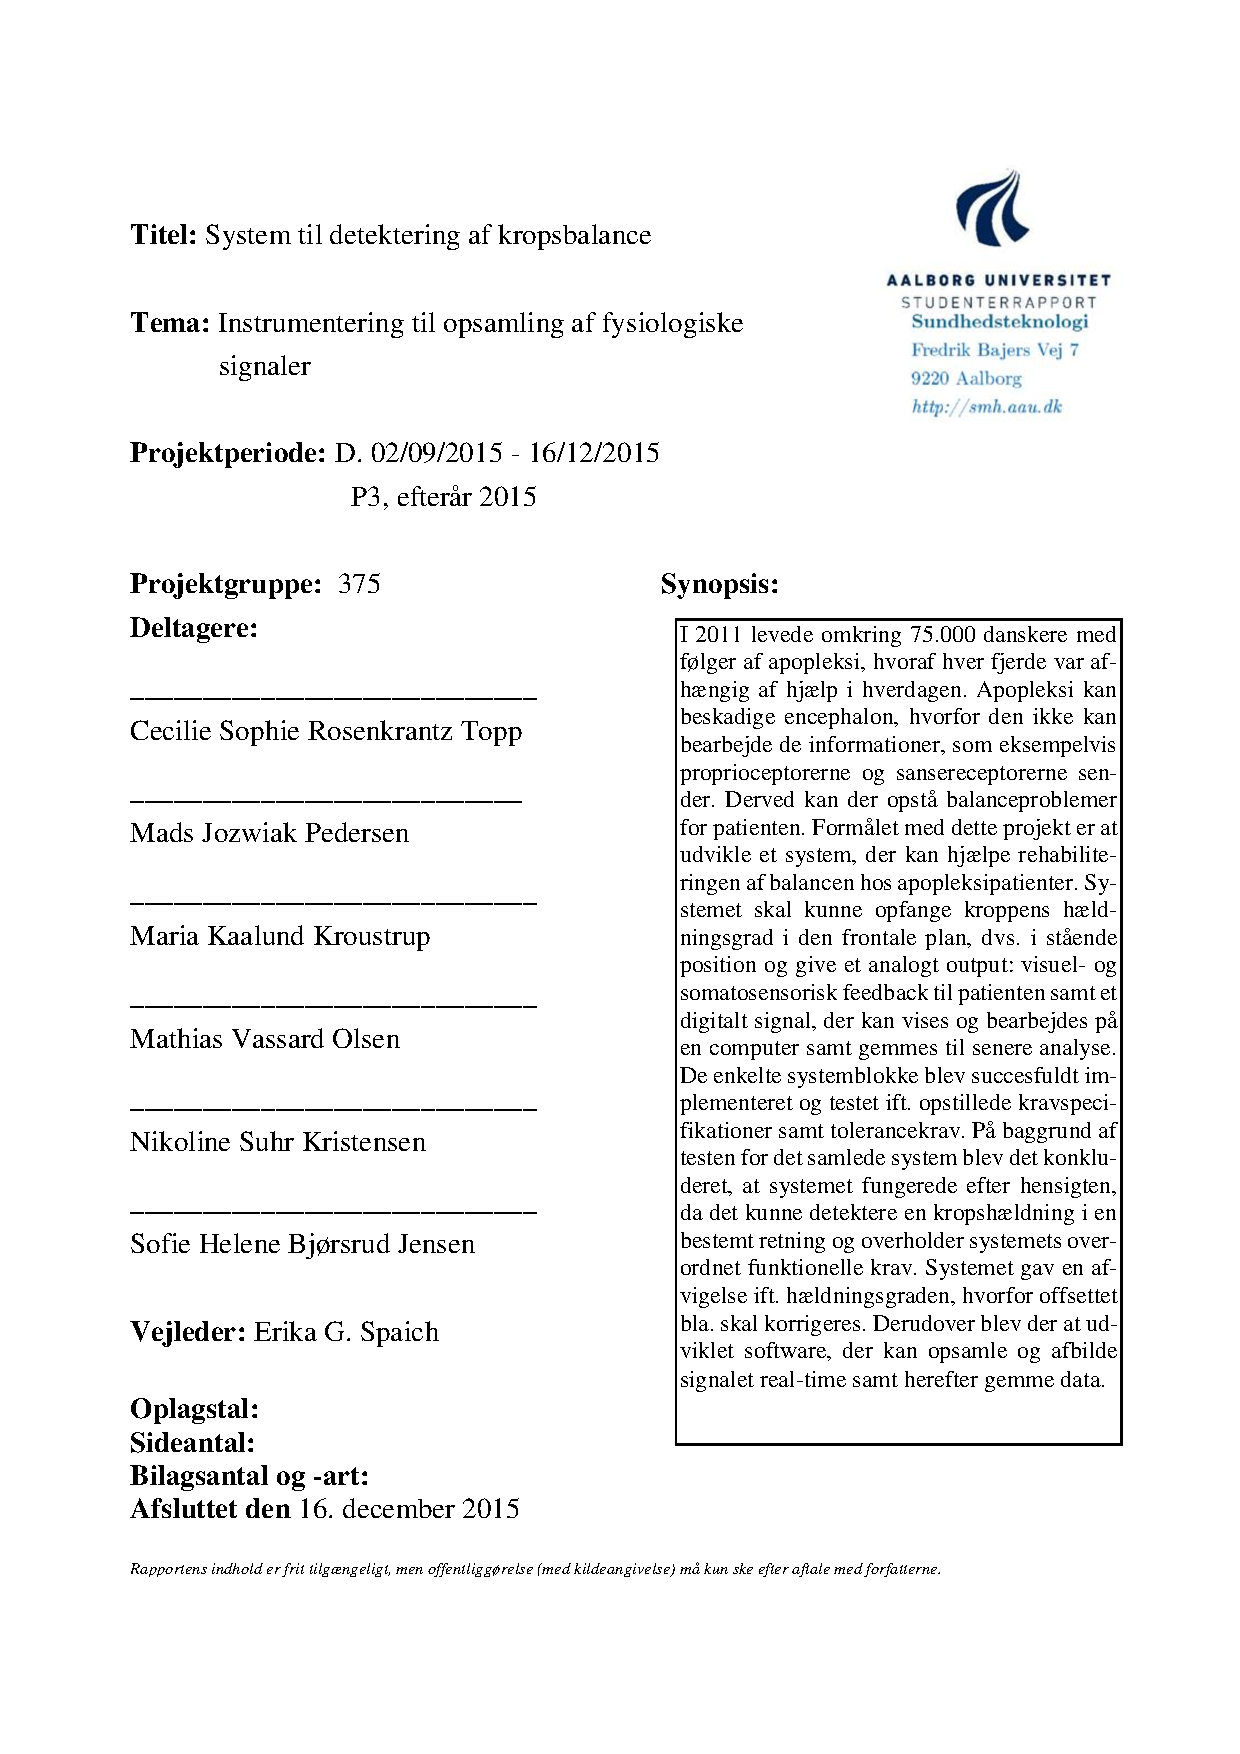
\includepdf[pages={1}]{rapportAfsnit/xFormaliteter/synopsis.pdf} 

% !TeX spellcheck = da_DK
\chapter*{Forord og læsevejledning}
\section{Forord}
Denne rapport er udarbejdet i forbindelse med et 3. semester projekt af studerende på Aalborg Universitet,  Sundhedsteknologi af gruppe 15gr375 i efteråret 2015. Ud fra projektets overordnede tema: "Instrumentering til opsamling af fysiologiske signaler" blev der heraf opstillet forskellige projektforslag. Denne rapport vil tage udgangspunkt i følgende projektforslag opstillet af Erika G. Spaich: "System til detektering af kropsbalance". Gruppens vejleder har under hele projektperioden været Erika G. Spaich.

Projektet rettes mod fagkyndigt personale, der beskæftiger sig med rehabilitering af apopleksipatienter og medstuderende på Aalborg Universitet, samt andre, der har interesse i emnet. 
Vi vil gerne takke vores vejleder Erika G. Spaich for vejledning og feedback igennem hele projektperioden. Derudover vil vi give en særlig tak til Jan Stavnhøj for hjælp og rådgivning til udarbejdelse af systemet samt Træningsenhed Vest Aalborg Kommune for at vi måtte komme og observere genoptræning af patienter med balanceproblemer. 

\section{Læsevejledning}
Projektrapporten er baseret på den problembaserede AAU-model. Selve rapporten er delt op i 4 kapitler, samt appendiks, således at første kapitel indeholder projektets initierende problem, der ligger til grund for problemanalysen. Andet kapitel indeholdende problemanalysen giver relevant viden om apopleksi og apopleksipatienternes følger, rehabiliteringsforløb og nuværende rehabiliteringsmuligheder, samt baggrundviden vedrørende teknologisk behandling af biologiske signaler.  Dette er efterfulgt af en projektafgrænsing samt problemformulering, der ligger til grund for problemløsningen. Problemløsningen beskrives i kapitel tre, indeholdende projektets praktiske del ift. at bygge et system til detektering af kropsbalancen. Herunder beskrives systemets kravspecifikationer samt systemdesign, herunder teori, simulering, implementering og test. I fjerde kapitel afsluttes rapporten med en evaluerende diskussion og konklusion af systemets funktion samt perspektivering ift. udvikling af systemet. Herefter findes litteraturlisten, samt appendiks, der henvises til som bilag A, bilag B osv. 

I rapporten benyttes Vancouver-metoden ved litteraturhenvisning, hvor anvendt litteratur tildeles fortløbende numre, således at den første reference i rapporten tildeles nummeret [1], den næste [2] osv. I litteraturlisten skrives den fulde reference, dvs. forfatter navn og årstal samt URL-kode hvis referencen er en hjemmeside, i den rækkefølge referencen anvendes i rapporten. Hvis referencen er placeret efter et punktum i en sætning tilhører referencen hele afsnittet, hvorimod er referencen placeret før et punktum tilhører referencen kun den pågældende sætning. Der der placeret flere referencer efter hinanden betyder dette, at der er anvendt flere referencer til den pågældende sætning eller afsnit. 

Derudover anvendes det amerikanske komma, når der i rapporten skrives tal, eksempelvis 12,500 og 2.4. Dvs. det amerikanske komma på dansk er et punktum og omvendt det amerikanske punktum på dansk er et komma.    

 \cleardoublepage

%the '*' allows the tableofcontents be excepted from the actual table of contents.
\tableofcontents*

%numbers the pages with Arabic numeral - starts from 1.
\mainmatter
\chapter{Indledning}\label{Indledning}
% !TeX spellcheck = da_DK
Apopleksi er pludselig opstået fokalneurologiske symptomer forårsaget af vaskulære forstyrrelser i hjernen, der kan forekomme pga. forhøjet blodtryk, diabetes eller rygning \cite{Sundhedsstyrelsen2009,Academic2015}. Apopleksi er den tredje største dødsårsag i Danmark og ca. 12.500 personer indlægges hvert år pga. sygdommen \cite{Hjernesagen2015a}. Andelen, der dør af hjerneskader, har været stagneret fra 2001 til 2011, hvor 14 \% døde inden for 30 dage \cite{Hjernesagen2015}. Derudover levede 75.000 danskere i 2011 med følger af apopleksi, og ud af disse er omkring hver fjerde person afhængig af hjælp for at kunne udføre dagligdagens gøremål \cite{Hjernesagen2015a}. Antallet af indlæggelsesforløb for mænd og kvinder stiger, når de bliver ældre end 65 år \cite{Sundhedsstyrelsen2011}.
Danskere der lever med følger og varige mén af apopleksi forventes at være stigende i takt med, at der kommer flere ældre \cite{Sagen2014}. Apopleksi er den sygdom, der kræver flest plejedøgn i sundhedssektoren. Ud fra et økonomisk perspektiv er det derfor dyrt for samfundet ift. omkostningerne til behandling, rehabilitering og produktivitetstab.  Udgifterne til sygdommen udgør 4\% af sundhedsvæsenets samlede udgifter, hvor direkte udgifter er estimeret til 2.7 milliard kroner om året \cite{Hjernesagen2015a, Kruuse2014}.
 
%I 2010 var der som sagt 18.041 indlæggelsesforløb forbundet med hjerneskade i Danmark, og det er langt fra alle, som slipper for varige mén heraf\cite{Sundhedsstyrelsen2011}. % gentagelse af det der skrevet før.
Følgerne af apopleksi opstår ofte pludseligt og kan både opleves som fysiske og mentale skader \cite{Muus2008}. Et af de hyppigste mén, som apopleksipatienter oplever, er neglekt. Patienter med neglekt er ikke opmærksomme på den ene side af kroppen \cite{Sundhed.dk}. Derudover opleves sensoriske- og motoriske skader herunder balanceproblemer. De nævnte følger har alle alvorlige konsekvenser for apopleksipatienters livskvalitet, da det bl.a. kan føre til  begrænsninger i hverdagen og i nogle tilfælde faldulykker. \cite{Muus2008,Nichols1997}

De fysiske- og mentale konsekvenser af sygdommen gør, det svært for en apopleksipatient at vende tilbage til sin normale hverdag. Problemer med balancen gør det f.eks. svært at udføre almindelige huslige pligter som rengøring og personlig pleje. \cite{Sundhedsstyrelsen2010} \\
Hjerneskadede patienter, heriblandt apopleksiramte, oplever nedsat livskvalitet pga. deres sygdom. Dette kan ses ved, at apopleksipatienter har dobbelt så stor selvmordsrate som baggrundsbefolkningen \cite{Sundhedsstyrelsen2010}. I en kvantitativ undersøgelse nævner 16\% af apopleksipatienter, at deres livskvalitet er dårlig	\fxnote{46\% nogenlunde, 38\% god} \cite{Sundhedsstyrelsen2010}. Den nedsatte livskvalitet kan føre til vanskeligheder senere i livet \fxnote{Måske skrive hvorfor}. En forbedret livskvalitet kan skabes ved hurtigere rehabilitering eller forbedret kropslige funktioner, som den apopleksiramte mistede ved hjerneskaden. \cite{Sundhedsstyrelsen2010}

For at patienterne opnår den bedst mulige behandling og rehabilitering er det afgørende, at der er et fungerende sammenspil mellem kommuner, sygehuse og praktiserende læger. Apopleksipatienter er krævende ift. rehabilitering pga. omfattende følger efter hjerneskaden. \cite{Sundhedsstyrelsen2010} Det er derfor vigtigt, at fokusere på patienternes rehabilitering for at kunne genoptræne de forskellige fysiske- og mentale mangler de oplever i dagligdagen samt give dem større livskvalitet. 

%Akut behandling og rehabilitering afhænger organisatorisk af hinanden, da sammenspillet mellem kommuner, sygehuse og praktiserende læger er afgørende. % Apopleksi har omfattende og alvorlige konsekvenser og der er derfor brug for involvering fra flere sundhedsprofessionelle områder.\cite{Sundhedsstyrelsen2010}
%De omfatende og alvorglige konsekvenser samt sammenspillet mellem sundhedsområder og rehabilitering er bl.a. det, som gør, at apopleksi er omkostningsfuldt for samfundet.\cite{Sundhedsstyrelsen2010} \\
%Apopleksi påvirker patienters livskvalitet og identitet, da det er svært for patienterne at forholde sig til sygdommen og derved påvirker deres humør, personlighed, færdigheder og sociale relationer. Det er derfor vigtigt at genoptræne patienterne ved at rehabilitering for, at de kan genfinde eller forbedre deres tabte funktioner, f.eks. ved brug af teknologier, som på denne måde er med til at genoprette identitet samt forbedre livskvaliteten for patienten.\cite{Sundhedsstyrelsen2010} 

%Det vil derfor kunne forventes, at der er flere, som kommer ud for en hjerneskade og vil have varige mén herefter, hvilket gør det vigtigt at fokusere på rehabiliteringen for at kunne genoptræne de forskellige kropslige- og mentale mangler.

%%%%%%%%%%%%%%%   Marias foreslag til indledning
%Det kræver samarbejde fra flere professionelle plejepersonale som kommuner, sygehuse og praktiserende læger for at give patienten den rette rehabilitering, da apopleksi patienter er omfattende og kan have alvorlige konsekvenser. Dette gør også at apopleksi er omkostningsfuldt for samfundet. 
% !TeX spellcheck = da_DK
\section{Initierende problem}
Hvilke fysiologiske konsekvenser kan apopleksi have for patienten, og hvad er rehabiliteringsmulighederne for en patient med balanceproblemer? 

%%%%%%%%%%%%%% FORESLAG TIL ANDRE INITIERNEDE PROBLEMER, DER ER MERE PROBLEMORIENTERET %%%%%%%%%%%%%
% 

\chapter{Problemanalyse}
\section{Apopleksi}

Et apopleksi tilfælde kan være forårsaget af enten en blodprop i hjernen (iskæmisk) eller hjerneblødning (hæmoragisk).
Apopleksi er af World Health Organization (WHO) defineret som pludseligt opstået fokale neurologiske symptomer pga. forstyrrelser i hjernens blodcirkulation, der varer mere end 24 timer eller fører til døden[1]. Hvis varigheden er under 24 timer, betegnes det som transitorisk cerebral iskæmi (TCI), hvor de fleste tilfælde varer under 1 time[2] uden permanent hjerneskade [3].

(Billeder)

Iskæmisk apopleksi forekommer hyppigst%ift. hvad? 
[2] og opstår, når en hjernearterie blokeres af en blodprop (infarkt), der stopper tilførslen af blod til et bestemt område i hjernen, hvilket ses på figur xx. Infarkterne dannes primært pga. åreforkalkning enten ved en trombe, der dannes på stedet, eller emboli fra hjertet. Nervecellerne skades efter få minutter pga. stoppet blodtilførsel og vil gå tabt [5].

Hæmoragisk apopleksi skyldes hovedsageligt forhøjet blodtryk eller i sjældnere tilfælde bristede svagheder på arterier (aneurismer) eller misdannede kar[5]. Hæmoragisk apopleksi opstår, når en hjernearterie brister og lækage af blod danner en blodansamling (hæmatom), der beskadiger det omkringliggende væv og forøger trykket i hjernen, hvilket ses på figur xx. Blødning i selve hjernen (intracerebral hæmoragi) kommer af forhøjet blodtryk, der danner et pres på de små arterier, som får dem til at briste[4] og forekommer i 10-12\% af tilfældene[2]. %ift. hvilke tilfælde? 
Blødning i rummet mellem de to hjernehinder (subaraknoidalrummet) skyldes bristning af et aneurisme på en pulsåre i hjernen [5] og forekommer 3-5\% af tilfældene[2]. Symptomerne ved subaraknoidalblødning er generel tab af hjernefunktion, da der forekommer et øget pres på hjerneskallen, hvorimod ved intracerebral hæmoragi er hæmatomet lokaliseret et bestemt sted i hjernen og forårsager nedsat funktion ved én bestemt hjernefunktion[4]. 

% WHO - find en dansk difination istedet.
% Fjern paranteserne - skrev enten det rigtige ord først eller lav en anden måde at skrive det på.
% Mangler lidt en forklaring på, hvordan og hvorfor apopleksi det opstår. Man kan godt uddybe mere i det, der allerede er skrevet.
% Når der er bygget mere på, kan man godt lave nogle forskellige overskrifter.
% Fakta omkring, hvad der er årsagen til apopleksi - hjertesagen har nogle forksellige info om det. Fakta om apopleksi.
% !TeX spellcheck = da_DK
\subsection{Påvirkning på encephalon}\label{HjerneSenMot}
Cerebrum er den største region af encephalon, hvor der sker en processering af sanserne, tale, tanker, synet, hukommelsen og følelser. \cite{Martini2012} Jævnfør afsnit \ref{IskaemiskApp}, side \pageref{IskaemiskApp} er $80$-$85\%$ af apopleksitilfældene iskæmiske og rammer hyppigst i media arterien, der forsyner det meste af cerebrum med blod. Derfor er det ofte sensoriske og motoriske områder, der skades ved et apopleksitilfælde. \cite{Sundhed.dk2014,Kruuse2015a,Gade2004,Boss2010} En yderligere beskrivelse af encephalons anatomi kan ses i bilag \ref{AppNerve} på side \pageref{AppNerve}. For at opretholde balancen kræves et samarbejde mellem de sensoriske og motoriske områder i encephalon, som ses på \figref{Enc}.

\begin{figure}[H]
	\centering
	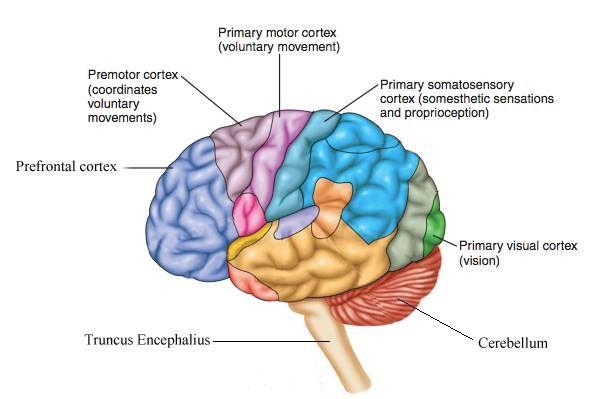
\includegraphics[scale=0.8]{figures/bProblemanalyse/Encephalon3.jpg}
	\caption{På figuren ses de sensoriske og motoriske regioner på den venstre hjernehalvdel af cerebrum. Derudover ses cerebellum og truncus encephalius. \textit{(Revideret)} \cite{Stanfield2014}}
	\label{Enc}
\end{figure}

\noindent De sensoriske og motoriske områder har indflydelse på hinanden. I \tableref{tabelencephalon} beskrives de områder i encephalon illustreret på \figref{Enc}, der har indvirkning på balancen samt funktionen af disse. Ved apopleksi kan flere områder blive beskadiget, hvilket kan medføre, at flere funktioner svækkes. Da balancen kontrolleres af flere forskellige områder i encephalon, betyder en skade på eksempelvis det visuelle cortex ikke, at balancen mistes helt. 

\begin{table} [H]
	\centering
  \begin{tabular}{ | l | p{10cm} |} \hline
    \textit{Område i encephalon} & \textit{Balancefunktioner} \\ \hline
 	Cerebellum & Modtager proprioreceptiv og vestibulær information fra medulla spinalis og truncus encephalius.  Fortolker og koordinerer frivillige bevægelser. \\ \hline
 	Det visuelle cortex & Fortolker lyssignaler, videresender informationer omkring rumlige forhold, bevægelse og koordinerer visuelle og somatosensoriske impulser. \\ \hline
 	Det præmotoriske cortex & Integrerer de sensoriske og motoriske systemer og igangsætter bevægelse som respons på visuelle eller auditive stimuli. \\ \hline
 	Det præfrontale cortex & Koordinerer information fra de andre cortex og udarbejder abstrakte intellektuelle funktioner som at forudse, hvilken effekt en handling vil have. Bearbejder eksterne sanseindtryk inden der foretages en handling. \\ \hline
 	Truncus Encephalius & Modtager vestibulær information fra det indre øre, som fortæller om hovedets placering i rummet og generel balance ift. til tyngdekraften. \\
    \hline
    \end{tabular}
    \caption{På tabellen ses en oversigt over de områder af encephalon, som påvirker balancen, samt deres funktioner. Områderne kan ses på \figref{Enc} \cite{Martini2012, Moos2010}}
    \label{tabelencephalon}
\end{table}
Nervebanerne fra hhv. sensorisk og motorisk cortex løber ned gennem medulla spinalis og leder derved impulser ud til targetorganer og muskler og tilbage igen. Nervebanerne fra hhv. højre og venstre hjernehalvdel krydser i medulla oblongata eller i medulla spinalis. Krydsningen medfører, at afferente signaler fra højre side af kroppen behandles i venstre hjernehalvdel, der sender efferente signaler tilbage til højre side af kroppen. \cite{Martini2012,Stanfield2014} Dette medfører, at et apopleksitilfælde i højre hjernehalvdel kan give sensoriske og motoriske skader i venstre kropsdel og omvendt for venstre hjernehalvdel. \cite{Nichols1997,Sundhedsstyrelsen2009} %Et apopleksitilfælde kan derved lede til neglekt eller problemer med balancen .

Hver muskelgruppe har sine egne dedikerede nerveceller. Antallet af nerveceller til hver muskel afhænger af, hvor kontrolleret muskelgruppens bevægelse skal være. Flere nerveceller øger præcisionen af musklens bevægelse. \cite{Stanfield2014} Nerveceller har en bestemt placering i cerebral cortex. Derfor vil et apopleksitilfælde et bestemt sted ramme en bestemt muskel. F.eks. vil en skade på det auditive cortex muligvis medføre balanceproblemer, da det derved er svært for patienten at vide, hvor hovedet er placeret i rummet. \cite{Mao2014} %Efter et apopleksitilfælde har encephalon en naturlig tilpasningsevne ift. at genskabe disse tabte funktioner. I nogle tilfælde kan encephalon genskabe skadede nerver eller finde en anden vej for funktionen, som en eventuelt tabt nerve skulle udføre. \cite{Martini2012} Denne mekanisme kaldes plasticitet \cite{Ramanathan2006}. 

\subsection{Plasticitet}
Efter et apopleksitilfælde har encephalon en naturlig tilpasningsevne ift. at genskabe disse tabte funktioner. Encephalon kan ændre eller tilpasse sig de stimuli, den udsættes for, hvilket kaldes encephalons plasticitet eller nerveplasticitet. Processen sker kontinuerligt igennem hele livet, men encephalon kan ikke danne nye nerver. \cite{Stanfield2014} Under et apopleksitilfælde forekommer der iltmangel til encephalon, hvilkens kan skader nervecellerne eller resultere i celledød \cite{Schulze2011}. Dette medfører, at den døde nerve mister sine forbindelser til fungerende nerver. Denne forbindelsesafbrydelse i encephalon bevirker, at der kan opstå en kaskade af mistet kommunikation i de eksisterende nerver. Herved kan en nerves celledød påvirke andre områder af encephalon end det sted, hvor skaden er sket. \cite{Raine2009} Encephalon benytter sig af sin plasticitet således, at omlægge det eksisterende nervenetværk til et nyt. Der aktiveres signalstoffer, som kan finde alternative metoder til at gennemføre den ønskede handling. \cite{Rugnett2015} Encephalon kan ikke danne nye nerver efter celledød, hvilket betyder, at der ikke kan generhverves præcis samme funktion som tidligere. En evt. lignende funktion kan generhverves ved gentagende træningsøvelser og kan deles op i følgende fænomener: \cite{Raine2009}

\begin{itemize}
	\item Denervation Supersensitivity: Sker ved en afbrydelse imellem akson og synapse og medfører, at synapsen bliver overfølsom og derved lettere påvirket til at indgå nye synapseforbindelser.
	\item Unmasking of Silent Synapses: Sker når synapser, der tidligere ikke havde en funktion, tilgås og der herved skabes nye funktioner.
	%Sker når synapser med fuld funktionalitet, men ingen effekt på slutstedet, afsløres, hvorefter der opstår en aktivitet og effekt. Dvs. synapsen fungerer, men encephalon er ikke opmærksom på dette.
	\item Collateral Sprouting: Sker hvis to nerver innerverer på samme slutsted, og den ene nerve dør, vil den anden nerve spire ind i den skadede nerves telodendron, så funktionen genvindes.
\end{itemize}

\noindent Ud fra disse fænomener findes der en fysiologisk baggrund for rehabilitering. Forekomsten af nerveplasticitet er særlig øget op til en måned efter et apopleksitilfælde. Det er derfor vigtigt at foretage genoptræning i denne periode, så encephalon kan danne nye forbindelser og kommunikationsveje. \cite{Rugnett2015} Gentagelser af en færdighed effektiviserer synapseforbindelser, hvilket betyder, at den kompenserende færdighed styrkes \cite{Stanfield2014}. En kompenserende færdighed dækker over de kompenserende bevægelser, som kroppen skaber for at erstatte en tabt funktionsevne \cite{Takeuchi2012,Leea2009}.

Nerveplasticitet betragtes ikke kun som en positiv egenskab. Plasticiteten gør encephalon fleksibel for omlægning efter en skade, men også sårbar overfor udefrakommende og interne ubevidste påvirkninger. Dårlige vaner er en negativ egenskab ved plasticitet, fordi gentagende hændelser, der frigiver dopamin, også giver stærke synapseforbindelser. Når mennesker forsøger at slippe af med en vane, som f.eks. rygning, vil det neurale kredsløb i encephalon blive svagere, men det findes stadig og kan genaktiveres, hvormed vanen kan genoptages. \cite{Hampton2015}

 %Udover plasticitet vil kroppen også skabe såkaldte kompenserende bevægelser for at erstatte en tabt funktionsevne. %Kompensatoriske bevægelser er et resultat af, at kroppen stadigvæk har brug for en givet funktion, men pga. tabt sensorisk og motorisk funktion ikke kan udføre bevægelsen. Disse kompenserende bevægelsesmønstre kan medføre et funktionelt dårligt resultat og kan være associeret med langsigtede konsekvenser såsom smerte og reduceret funktionsevne \cite{Takeuchi2012,Leea2009}.


%\subsection{Plasticitet}
%Encephalon kan ændre eller tilpasse sig de stimuli, den udsættes for, hvilket kaldes encephalons plasticitet eller nerveplasticitet. Dette sker kontinuerligt igennem hele livet, men encephalon kan ikke danne nye nerver. \cite{Stanfield2014} Under et apopleksitilfælde forekommer der iltmangel til encephalon, og nervecellerne kan derved blive skadet eller gå tabt. \cite{Schulze2011} Denne celledød gør, at den døde nerve mister sine forbindelser til raske nerver. Denne forbindelsesafbrydelse i encephalon bevirker, at der kan opstå en kaskade af mistet kommunikation i de eksisterende nerver. Herved kan en nerves celledød altså påvirke andre områder af encephalon end blot der, hvor skaden er sket. \cite{Raine2009} Encephalon vil benytte sig af sin plasticitet og omlægge det eksisterende nervenetværk. Encephalon vil aktivere nogle signalstoffer, som kan finde en alternativ metode til at gennemføre den ønskede handling. \cite{Rugnett2015}  Som sagt kan encephalon ikke danne nye nerver efter celledød, hvilket betyder, at der ikke kan generhverves præcis samme funktion som tidligere men evt. en lignende funktion. Men encephalon vil forsøge at kompensere for de tabte nerver ved at danne nye forbindelser og kommunikationsveje, hvilket kan deles op i tre fænomener: \cite{Raine2009}

%\begin{itemize}
	%\item En afbrydelse imellem akson og synapse medfører, at synapsen bliver overfølsom og derved lettere påvirket til at lave nye synapseforbindelser. Dette fænomen kaldes “Denervation Supersensitivity”.
%	\item Synapser, der har fuld funktionalitet men ingen effekt på slutstedet, “afsløres”, hvorefter der opstår en aktivitet og effekt. Dette kaldes “Unmasking of Silent (Latent) Synapses”.
%	\item Hvis to nerver innerverer på samme slutsted, og den ene nerve dør, så vil den anden nerve spire ind i den skadede nerves telodendron, og funktionen vil derved genvindes. Dette kaldes “Collateral Sprouting”.
%>>>>>>> origin/master
%\end{itemize}

%det forrige
%\subsection{Påvirkning på encephalon}\label{HjerneSenMot}

%Cerebrum er den største region af encephalon og kan deles op i to hjernehalvdele. Her sker en processering af sanserne, tale, tanker, synet, hukommelsen og følelser. \cite{Martini2012} For en yderligere beskrivelse af hjernen, nervefysiologi samt biologisk kommunikation se bilag \ref{AppNerve}. De forskellige sensoriske- og motoriske regioner kan ses på \figref{Enc}. Som tidligere nævnt i afsnit \ref{IskaemiskApp} er 80-85\% af apopleksitilfældene iskæmiske og rammer hyppigst i media arterien, der forsyner det meste af cerebrum med blod. Derfor er det ofte sensoriske- og motoriske områder, som bliver skadet ved et apopleksitilfælde. \cite{Sundhed.dk,Gade2004,Boss2010} \\

%\begin{figure}[H]
%	\centering
%	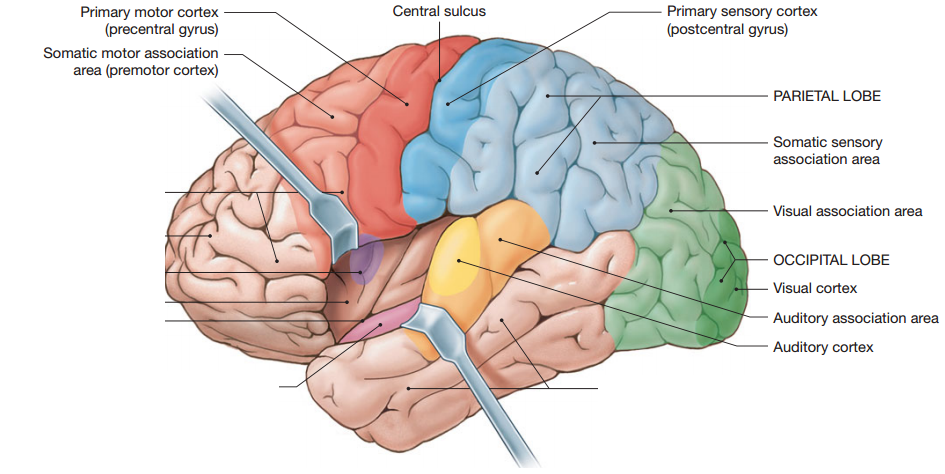
\includegraphics[scale=0.6]{figures/bProblemanalyse/Encephalon.png}
%	\caption{På figuren ses de sensoriske og motoriske regioner på den venstre hjernehalvdel af cerebrum. %\textit{(Revideret)} \cite{Martini2012}}
%	\label{Enc}
%\end{figure}

%De sensoriske- og motoriske nervebaner fra sensorisk- og motorisk cortex løber ned gennem medulla spinalis og leder derved impulser ud til target organer og muskler og tilbage igen. Nervebanerne fra hhv. højre og venstre hjernehalvdel krydser i medulla oblongata eller i medulla spinalis. Denne krydsning betyder, at afferente signaler fra højre side af kroppen behandles i venstre hjernehalvdel, der sender efferente signaler tilbage til højre side af kroppen. \cite{Martini2012,Stanfield2014} Dette medfører, at et apopleksitilfælde i højre hjernehalvdel kan give sensoriske- og motoriske skader i venstre kropsdel og omvendt med venstre hjernehalvdel. \cite{Sundhedsstyrelsen2009,Nichols1997} %Et apopleksitilfælde kan derved lede til neglekt eller problemer med balancen .

%Hver muskelgruppe har sine egne dedikerede nerveceller. Antallet af nerveceller til hver muskel afhænger af, hvor præcis legemets bevægelse skal være. Flere nerveceller gør musklens bevægelse mere præcis. \cite{Stanfield2014} Nervecellerne har en bestemt placering i cerebral cortex. Derfor vil et apopleksitilfælde et bestemt sted ramme en bestemt muskel. F.eks. vil en skade på det auditive cortex kunne medføre balanceproblemer, da det derved er svært for patienten at vide hvor hovedet er placeret i rummet. \cite{Mao2014} 
%\begin{center}
%\begin{tabular}{ | l | p{8cm} |}
%\hline
%Auditive cortex & hej med dig \\ \hline
%\end{tabular}
%\end{table}

%\subsection{Encephalons påvirkning på balance}
%For at opretholde balancen kræves der samarbejde af flere områder af encephalon. Disse har en stor indflydelse på hinanden. Områderne kan ses i \tableref{tabelencephalon}. Ved apopleksi kan flere områder rammes samtidig, hvilket kan gøre at flere funktioner svækkes. Da balancen er styret af flere forskellige områder i encephalon betyder en skade på eksempelvis det visuelle cortex ikke at man mister balancen helt. 

%\begin{center}
%\begin{table} [H]
  %\begin{tabular}{ | l | p{8cm} |}
   % \hline
  %  \textbf{Område i encephalon} & \textbf{Funktioner} \\ \hline
 %	Cerebellum & Modtager proprioreceptiv og vestibulær information fra medulla spinalis og truncus encephalius.  %Fortolker og koordinerer frivillige bevægelser. \\ \hline
 %	Det visuelle cortex & Fortolker lyssignaler og videresender informationer omkring rumlige forhold, bevægelse og %koordinerer visuelle og somatosensoriske impulser. \\ \hline
 %	Det præmotoriske cortex & Integrerer den sensoriske og motoriske systemer og igangsætter bevægelse som respons på %visuelle eller auditive stimuli. \\ \hline
 %	Det præfrontale cortex & Koordinerer information fra de andre kortex og udarbejder abstrakte intellektuelle %funktioner, som at forudse hvilken effekt en handling vil have. Bearbejdere eksterne sanseindtryk inden der foretages %en handling. \\ \hline
 %	Truncus Encephalius & Modtager vestibulær information fra det indre ører, som fortæller hovedets placering i %rummet og generel balance ift. til tyngdekraften. \\
    %\hline
   % \end{tabular}
 %   \caption{Tabel over de områder af encephalon som påvirker balancen, samt deres funktion. \cite{Martini2012, %Moos2010}}
 %   \label{tabelencephalon}
%\end{table}
%\end{center}


%Encephalon har en naturlig tilpasning. Dette medfører, at den i nogle tilfælde kan genskabe skadede nerver eller finde en anden vej for funktionen, som en eventuelt tabt nerve skulle udføre. \cite{Martini2012} Denne mekanisme kaldes plasticitet \cite{Ramanathan2006}.
% !TeX spellcheck = da_DK
\section{Behandlinger}
Når en patient rammes af apopleksi, er det vigtigt at komme i behandling hurtigst muligt. Ved ankomst på sygehuset foretages der en scanning af encephalon for at undersøge, hvorvidt det er iskæmisk eller hæmoragisk apopleksi. Hvis hæmoragisk apopleksi findes der endnu ingen akut behandling, der kan stoppe blødningen.\cite{Soenderborg2013} Hvorimod ved akut iskæmisk apopleksi, hvilket vil sige at symptomerne er til stede inden for fire en halv time, anvendes blodpropopløsende medicin. Ved hurtig behandling vil det være muligt at opløse blodproppen. I andre tilfælde fjernes blodproppen ved brug af et tyndt kateter, som indføres gennem arterien op til encephalon. Derudover anvendes blodfortyndende medicin for at undgå nye tilfælde af apopleksi. \cite{Hjerteforeningen2014, Kruuse2014a} 

%\subsection{Akut behandling}
%Ved mistanke om iskæmisk apopleksi er det vigtigt, at der tages kontakt til sygehuset omgående. Patienten bliver her undersøgt ved blodtryksmåling, blodprøver, neurologisk undersøgelse og scanning af encephalon. Dermed kan det udelukkes om der er eventuelle blødninger eller andre årsager til funktionstabet. Dette  sikrer, at patienten får den rette behandling. I tilfælde af blodprop igangsættes en behandling med blodpropopløsende eller blodpropshæmmende medicin. \cite{Hjerteforeningen2014, Kruuse2014a} 
%
\subsection{Trombolyse}
Standardbehandling for blodpropper har siden år 2006 været trombolyse. Selve behandlingen foregår ved, at der sprøjtes blodpropopløsende medicin ind i en arterie, ofte i armen, hvorefter blodproppen opløses. Denne behandling skal helst foregå seks timer efter blodproppens forekomst og senest 12 timer efter, da behandlingen ikke vil have nogen indvirkning efter længere tid. Hurtig behandling vil betyde at flere områder af encpehalon vil kunne reddes. Dermed vil patientens fremtidige livskvalitet forbedres. Trombolysebehandlingen finder sted på 12 sygehuse fordelt over de fem regioner. En risiko ved behandlingen kan være blødninger grundet den blodpropopløsende medicin. \cite{Hjernesagen2015b}

\subsection{Forebyggelse}
En væsentlig del af behandlingen er forebyggelse, da risikoen for en ny blodprop er betydelig. Til forebyggelse anvendes antikoagulationsbehandling, som er en behandling med blodfortyndende medicin. Normalt har kroppen sit eget koagulationsssystem som får blodet til at koagulere. Derudover medvirker koagulationssystemet også til at opløse evt. blodpropper i det kardiovaskulæresystem. For apopleksipatienter fungerer koagulationssystemet ikke optimalt, hvilket gør det nødvendigt at behandle med antikoagulation. Dette hæmmer blodets evne til at koagulere, hvilket modvirker dannelsen af blodpropper. Der findes to former for antikoagulationsbehandling, warfarin og nyre orale antikoaglulantia. Den primære forskel mellem de to mediciner er, at der ved behandling med nyre orale antikoaglulantia ikke kræves kontrol ved blodprøver.\cite{Kjaergaard2015}

%[1]http://www.hjerteforeningen.dk/alt-om-dit-hjerte/hjerte-kar-sygdomme/apopleksi/
%[2]http://www.hjernesagen.dk/om-hjerneskader/behandling/trombolyse
%[3] https://www.sundhed.dk/borger/sygdomme-a-aa/hjerte-og-blodkar/sygdomme/apopleksi/behandling-ved-apopleksi/
%[4]https://www.sundhed.dk/borger/sygdomme-a-aa/hjerte-og-blodkar/sygdomme/behandlinger/antikoagulationsbehandling-blodfortyndende-medicin/
\input{rapportAfsnit/cProblemanalyse/Foelger}
% !TeX spellcheck = da_DK
\section{Rehabilitering}
Når selve slagtilfældet er stabiliseret og behandlet, er det essentielt, at rehabiliteringen af en apopleksipatient indfindes hurtigst muligt - gerne en til to dage efter slagtilfældet. I Danmark dækker rehabilitering af en patient med apopleksi områderne: direkte træning af funktioner, ufrivillig reorganisering af hjernen netværk, kompenserende strategier, ændringer i miljø, social og psykologisk støtte. Genoptræningen omhandler dog ikke kun træning med en ergo- eller fysioterapeut, da plejepersonale til dagens almindelige gøremål også essentiel. Patientens daglige rutiner kan være gået tabt under slagtilfældet, hvorfor det er vigtigt, at få patienten tilbage i sit vante miljø. Plejepersonale skal hjælpe patienten til at genfinde denne rytme og hjælpe patienten til eventuelt at udføre dagligdags ting på en ny måde. Det kan ske, at patienten ikke længere er i stand til at beherske begge sine hænder til en opgave, hvorved plejepersonalet skal bistå patienten i indlæringen af kun at benytte en hånd.

Motoriske og sensoriske funktionsproblemer kan lede til balancebesvær for patienten i både siddende, stående og gående stilling. Der er afprøvet adskillige farmakologiske midler og behandlingsstadegier for at forbedre hjernens rehabilitering og motoriske funktioner. F.eks. er der afprøvet, at tildele apopleksipatienter det antidepressive middel fluoxetin i kombination med fysioterapi. Derudover er kortikal stimulation afprøvet, hvor området af hjernen, som kontrollerer motorstyring, modtager elektriske impulser fra en implanteret anordning. Denne mulighed har haft blandede succesoplevelser, men er udelukkende afprøvet på patienter, der har oplevet et alvorligt slagtilfælde. \cite{Academic2015}
  
Apopleksi patienten skal i samarbejde med lægen, sygeplejersken og andet hjælpepersonale opstille nogle mål for sin rehabilitering. Målene skal hverken være for svære eller for lette, så patienten ikke mister sin motivation til genoptræningen. \cite{Kruuse2015}

\subsection{Forløbsprogram for rehabilitering} 
Sundhedsstyrelsen har udarbejdet et forløbsprogram for rehabilitering af patienter med erhvervet hjerneskade. Forløbsprogrammet strækker sig fra at patienten erhverver hjerneskaden til at patienten har opnået bedst mulig funktionsevne, hvorefter der udføres kontrol og vedligeholdelse af funktionsevnen. Tidsperioden af rehabilitering varierer ift. hjerneskadens sværhedsgrad, samt sværhedsgraden af funktionstabet. %dog kan perioden vare flere år.  
\cite{Sundhedsstyrelsen2011a}

Forløbsprogrammet er essentielt i forhold til at kunne give patienten den korrekte rehabilitering. Patienterne har forskellige behov og er afhængige af hjælp fra plejepersonale. Deruodver kræves der forskellige former for teknologi i de forskellige faser. Det vil derfor være oplagt at undersøge, hvilken form for rehabilitering der er at foretrække i de enkelte faser som ses på \figref{firefaser}.

\begin{figure}[H]
	\centering
	\includegraphics[scale=0.6]{figures/bProblemanalyse/flowdiagram_faser1.png}
	\caption{På figuren ses et overblik over de fire faser, som patienter med apopleksi skal igennem i forløbsprogrammet for rehabilitering \cite{Sundhedsstyrelsen2011a}} 
	\label{firefaser}
\end{figure}

\subsubsection{Den første fase}
Som det vises på \figref{firefaser} afspejler første fase den del af forløbsprogrammet som foregår på sygehusets apopleksiafdeling. På apopleksiafdelingen foretages primært akut behandling for at begrænse skaderne. Når patientens sikkerhed er sikret og skaderne er begrænset påbegyndes den tidlige rehabilitering. Under den tidlige rehabilitering giver en speciallæge i neurologi en vurdering af patientens rehabiliteringsbehov. Derudover bliver patienterne overvåget i forhold til bevidsthed, ændringer og amnesi samt foretaget vurderinger af basale fysiologiske funktioner. Samtidig bliver der iværksat træning i diverse bevægelsesfunktioner, basale egenskaber og kommunikationsfunktioner. Patienterne gennemgår også en tidlig behandling og diagnostik for at undersøge komplicerende tilstande, som f.eks. vaskulære hændelser, blodpropper i ben og lunger og smerter. Patienterne vurderes i denne fase af fagkyndigt personale som ergoterapeut, fysioterapeut og audiologopæd \fxnote{høre og talepædagog}. Disse er med til, at sikre, at patienten udfører træningen korrekt i forhold til stilmulering og træning af bevægelsesfunktioner, taletræning og udførsel af basale daglige aktiviteter.\cite{Sundhedsstyrelsen2011a}

\subsubsection{Den anden fase}
Det fremgår af \figref{firefaser}, at patienten i den anden fase gennemgår rehabilitering på sygehuset, hvor der er fokus på de skadede funktioner. Ligeledes bliver patienten på samme måde som i fase et undervist af fagkyndigt personale. Hvorefter patientens behov for rehabilitering og rehabiliteringens udvikling vurderes. Patienterne bliver i denne fase udredet i forhold til funktionsevne, mentale funktioner, bevægelsesfunktioner herunder bevægelse og mobilitet i led, knogler, reflekser og muskler samt rehabilitering med henblik på daglige aktiviteter. Hvis patienten vurderes til at have en stabil udvikling i rehabiliteringsprocessen, vil patienten blive udskrevet og påbegynde fase tre. \cite{Sundhedsstyrelsen2011a}


\subsubsection{Den tredje fase}
I den tredje er patienten udskrevet fra sygehuset. Derved foregår rehabilitering som ambulant rehabilitering og selvstændig træning, som det fremgår af \figref{firefaser}.  Selve rehabiliteringen i tredje fase er bygget op ud fra rehabiliteringsforløbet i den anden fase. Det afgørende for den tredje fase er, hvorvidt patienten skal vedblive rehabilitering på sygehuset eller henvises til de kommunale rehabiliteringscentre. Dette afgøres på baggrund af observationer foretaget i anden fase. Den selvstændige træning kan for patienter med neglekt og balanceproblemer være en udfordring ift. bevægelsesmønstre og kropsholdning. \cite{Sundhedsstyrelsen2011a}

\subsubsection{Den fjerde fase}
Det fremgår på \figref{firefaser}, at fjerde fase er den afsluttende fase for behandlingsforløbet. Patienterne går stadig til kontrol og vedligeholdelse for at sikre, at rehabiliteringens udvikling er stabil. Det kan i sidste ende have betydning for, hvor lang tid det tager for patienten at generhverve sine tabte funktioner. Den fjerde fase varierer derfor fra patient til patient alt efter udviklingen af rehabiliteringen.\cite{Sundhedsstyrelsen2011a} \\

\subsection{Organisatorisk}
Sygehusvæsenet, almen praksis og kommuner har opgaver i alle faser, dog i varierende grad. Således har sygehuset flest opgaver i fase I og II, mens kommunen og almen praksis har flest opgaver i fase III (og IV) \cite{Sundhedsstyrelsen2011a}.

%\section{Organisatorisk}
%I sundhedssektoren arbejder de forskellige organisatoriske aktører på tværs af hinanden. Der er således et samarbejde mellem syghuse, kommuner og praktiserende læger. Dette samarbejde skal ske både internt på syghusene, på afdelingerne og kommunalt mellem forvaltningerne \cite{Sundhedsstyrelsen2010}. Samspillet mellem aktørerne er vigtigt, da patienter med hjerneskade berører flere afdelinger. De har derfor brug for involvering af flere sundhedsprofessionelle grupper under behandling og rehabilitering på grund af de omfattende og alvorlige konsekvenser.

%De ovennævnte aktører er de organisatoriske enheder, der har en central rolle i forløbet. Det er ikke muligt at fastlægge en egentlig organisering af hjerneskaderehabiliteringen i Danmark, da sammenspillet mellem de forskellige aktører er meget flydende og forskellige alt efter hvor i landet man befinder sig og hvor omfattende hjerneskaden er. Denne forskel opleves regionalt, hvor behandling og rehabilitering enkelte steder foregår på få af sygehusets afdelinger, mens patienter andre steder behandles på et rehabiliteringssygehus, efter den akutte behandling er foretaget.\cite{Sundhedsstyrelsen2010}

%I starten af behandlingssforløbet sendes patienterne til neurologiske, geriatriske, neurokirurgiske og medicinske afdelinger på sygehuset. Som tidligere nævnt inddeles patienterne efter sværhedsgrad af hjerneskaden, hvor de sværest ramte, som er patienter med traumatisk hjerneskade og tilgrænsede lidelser, vidererstilles til Hammel og Hvidovre. Rehabiliteringen kan også ske på rehabiliteringsafsnittene på landets sygehuse.
%Det primære ansvar ligger hos kommunerne i form af genoptræningsplanens afdækning af rehabiliteringsbehov, dvs. at kommunerne holder øje med om dette foregår i praksis, herunder bl.a. patientens genoptræningsbehov. Kommunen har derudover mulighed for at henvise patienterne til dens egne tilbud, samt at henvise til private.\cite{Sundhedsstyrelsen2010} 

%Afslutningsvis gennemgår patienterne et langt og forskelligt behandlingsforløb alt efter hjerneskadens omfang. Forløbet indebærer et samarbejde mellem de forskellige aktører. Efter behandlingen står kommunerne, som førnævnt, for det primære ansvar i forhold til rehabilitering og henvisning for patienten\fxnote{hvor kommer denne info fra?}.



% I første og anden fase af rehabiliteringsforløbet bliver patienten undervist og overvåget af fagkyndigt personale. Dette gøres for at sikre, at patienten udfører træningen korrekt f.eks. med bevægelsesmønstre, og korrigere patienten til at bevægelsen og øvelserne udføres korrekt. Dette er vigtigt, da patienten, som sagt i tredje fase, selv skal foretage den nødvendige træning og dermed har fornemmelse af, hvordan træningen udføres korrekt ift. bevægelsesmønstre og kropsholdning. Dette kan midlertidig være en udfordring for apopleksipatienter med neglekt, da de kan have problemer med balancen og opmærksomheden på kroppen. Patienten går derfor stadig til kontrol og vedligeholdelse for at sikre, at rehabiliteringens udvikling er stabil. Det kan i sidste ende have betydning for, hvor lang tid det tager for patienten at generhverve sine tabte funktioner. Den tredje fase varierer derfor fra patient til patient alt efter udviklingen på rehabiliteringen. \cite{Sundhedsstyrelsen2011a}
% !TeX spellcheck = da_DK
\subsection{Nuværende metoder til rehabilitering}

Inden patienten udskrives fra sin behandling skal der fra sundhedssektorens side være udarbejdet en genoptræningsplan. I denne plan besluttes det hvilken form for rehabilitering og teknologi patienten skal benytte sig af. \cite{Sundhedsstyrelsen2011a} \\
Der findes flere forskellige metoder og teknologier til at hjælpe med balance og gangproblemer. Disse omfatter: Platform feedback, fokuseret gangtræning, konditionstræning, auditorisk rytmestøtte, elektromekanisk fysioterapistøttet gangtræning, opgavespecifik repetitiv træning, spejlterapi, programmer til motorisk visualisering og passiv sensorisk stimulation. \cite{Sundhedsstyrelsen2011a}\fxnote{dette skal laves om til punktform.} \\
Platform feedback er en biofeedback metode, hvor patienten står på en platform. Platformen vil herefter måle hvor meget patienten svajer \fxnote{(centre of pressure)}. Når platformen har målt svajningen af patienten, kan denne enten få visuel eller auditiv feedback. Feedbacken skal gøre patienten mere opmærksom på, hvor meget kroppen svajer, hvilket gør det muligt at opretholde en stående position.%[1]
Denne form for teknologi benyttes særligt i de tidlige faser af rehabiliteringen\cite{Sundhedsstyrelsen2011a}. \\
Det er med høj evidens blevet påvist, at fokuseret gangtræning medfører en moderat grad af bedringen på gangfunktionen hos apopleksiramte\cite{Sundhedsstyrelsen2010}. Derudover er det også vist, at konditionstræning kan være med til at forbedre gangfunktionen\cite{Sundhedsstyrelsen2010}. \\
Auditorisk rytmestøtte er en metode, hvor patienten lytter eller udfører handlinger til en form for musik. Det mest centrale ved musikken er rytmen, der findes i den.%[2] 
Det er vist, at denne metode kan øge både ganghastigheden, skridtlængden og gangsymmetrien \cite{Sundhedsstyrelsen2010}. \\
Ved elektromekanisk fysioterapistøttet gangtræning benytter fysioterapeuten sig af en maskine til hjælp af patientens gang. Maskinen består af enten et robot-drevet exoskelet eller to drevne mekaniske plader, der simulerer gang hos patienten. %[3] 
Denne form for metode har vist at kunne øge skridthastighed, skridtlængde og skridtsymmetri \cite{Sundhedsstyrelsen2010}. Denne metode benyttes til patienter med svært nedsat gangfunktion, med særlig fokus på de tidlige faser af rehabiliteringen \cite{Sundhedsstyrelsen2011a}. \\
Opgavespecifik repetitiv træning omfatter aktivitetsbestemte motoriske opgaver, som er bestemt til den enkelte patient. Disse opgaver tager udgangspunkt i hverdagsaktiviteter. Denne metode kan have effekt på patienternes gangfunktion, gangdistance og -hastighed. \cite{Sundhedsstyrelsen2010} \\
Spejlterapi er en træning af bevægelser, hvor patienten laver en række bevægelsesmønstre med den raske side af kroppen. Herefter bliver disse bevægelser spejlet til den syge side af kroppen. Dette vil skabe en illusion af et normalt bevægelsesmønster af den syge side hos patienten. \cite{Sundhedsstyrelsen2010} Denne metode skal tilbydes under hele rehabiliteringen \cite{Sundhedsstyrelsen2011a}.\fxnote{Måske uddybe, hvordan spejlingen foregår..} \\
Programmer til motorisk visualisering kan bl.a. være "virtual reality" \cite{Sundhedsstyrelsen2010}. Dette er en form for program, hvor en computer modellerer og simulerer et miljø, som patienten kan placeres i vha. briller og andre interaktive apparater[4]. Dette gør at patienten kan simulere bevægelser, som de ikke nødvendigvis er i stand til i virkeligheden. Det er uafklaret, hvilken effekt denne form for rehabilitering har \cite{Sundhedsstyrelsen2010}. \\
Passiv sensorisk stimulation er en rehabiliteringsform, hvor patienten modtager elektrisk stimulation, der ikke aktiverer musklerne. Stimulationen er der for at fortælle patienten om, hvad kroppen foretager sig, så det bliver muligt at korrigere bevægelserne. \cite{Sundhedsstyrelsen2010} Denne form for metode tilbydes under hele rehabiliteringsforløbet \cite{Sundhedsstyrelsen2011a}.\fxnote{Dette må også gerne uddybes - hvordan har det en gavnlig effekt at ens muskler ikke aktiveres?}
%
%
%[1] - http://onlinelibrary.wiley.com.zorac.aub.aau.dk/doi/10.1002/14651858.CD004129.pub2/full
%[2] - http://onlinelibrary.wiley.com.zorac.aub.aau.dk/doi/10.1002/14651858.CD006787.pub2/full
%[3] - http://onlinelibrary.wiley.com/doi/10.1002/14651858.CD006185.pub3/full
%[4] - http://academic.eb.com.zorac.aub.aau.dk/EBchecked/topic/630181/virtual-reality-VR/
\input{rapportAfsnit/cProblemanalyse/biofeedback}
% !TeX spellcheck = da_DK
\section{Behandling af kropshældnings signal}
Et biologisk signal skal behandles for at kunne give feedback til patienten samt et digitalt output evt. til plejepersonale. For at kunne behandle et signal fra et accelerometer kræves der bl.a. forstærkning, filtrering, komparator samt ADC. Der kan anvendes andre komponenter til signalbehandling ift. hvad accelerometret skal benyttes til, men de nævnte vil blive benyttet i dette projekt. 

\subsection{Forstærker}\label{forstaerkerafsnit}
En forstærker kan benyttes til at ændre inputtet i form af et biologisk signal til et skaleret output. Dette kan gøres ved at kombinere en operationsforstærker med modstande, der derved kan skalere, invertere, addere og subtrahere signalet. Der findes fire forskellige forstærkningskredsløb til at udføre de nævnte opgaver: \cite{Nilsson2011}
\begin{itemize}
\item Inverterende forstærkningskredsløb: Benyttes til at invertere signalet samtidig med det skaleres.% Inverteringen af signalet betyder, at der ændres fortegn på signalet.
\item Summerende forstærkningskredsløb: Fungerer ligesom det inverterende forstærkningskredsløb med den undtagelse, at inputsignalerne summeres.
\item Ikke-inverterende forstærkningskredsløb: Benyttes til at skalere input signalet.
\item Differens forstærkningskredsløb: Benyttes til at trække to input signaler fra hinanden, så outputsignalet bliver forskellen på de to inputsignaler \cite{Nilsson2011}. Der findes forskellige typer af differensforstærkning, herunder et kredsløb med en enkelt operationsforstærker eller en instrumenteringsforstærker. I instrumenteringsforstærkeren indgår yderligere to operationsforstærkere for at lave inputbuffere til den oprindelige operationsforstærker. \cite{Sedra2010}  
\end{itemize} 

%\noindent For at forstærke signalet fra et accelerometeret benyttes operationsforstærkeren, der skalerer inputspændingen til en ønsket outputspænding. Dette gøres, hvis den næste komponent skal bruge et specifikt input eller for at forstærke signaler med lav amplitude. Der kan f.eks. bruges en inverterende forstærker, som ses på \figref{invf}, hvor $V_{s}$ er det målte signal, der ønskes forstærket og $V_{o}$ er outputsignalet. Inputtets forstærkning kaldes gain og er en ratio mellem $dfrac{R_{f}}{R_{s}}$, som er de to modstande. \cite{Nilsson2011}
%
%\begin{figure}[H]
%\centering
%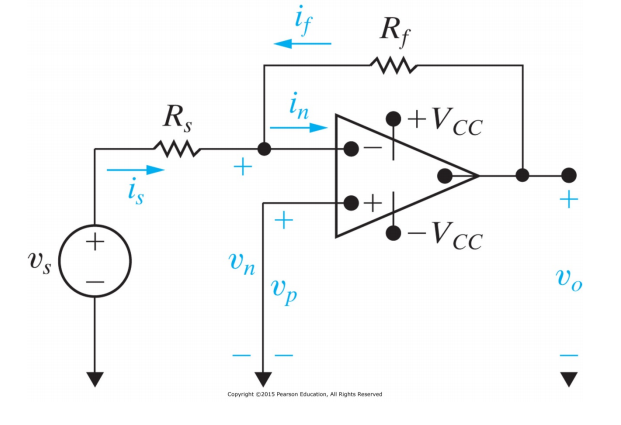
\includegraphics[scale=0.6]{figures/bProblemanalyse/inverterendeforstaerker.png}
%\caption{På figuren ses en ideel operationsforstærker, som er inverterende koblet og kan forstærke input signalet $V_{s}$ til et ønsket output signal $V_{o}$ vha. modstandene $R_ {s}$ og $R_{f}$. \cite{Nilsson2011}}
%\label{invf}
%\end{figure}


%INDLEDE MED KORT FORKLARING PÅ HVAD EN FORSTÆRKER EGENTLIG ER OG HVILKE FORSKELLIGE TYPER DER FINDES
%UNDERSTREGE AT VI GODT VED AT DER ER FLERE FORSKELLIGE TYPER AF FORSTÆRKERE..
% !TeX spellcheck = da_DK
\subsection{Filtrering}
Filtrering er et værktøj indenfor databehandling, som anvendes i det målte signals frekvensdomæne. Formålet med at filtrere et målt signal er at fjerne uønskede frekvenser, også kaldet støj, der ikke tilhører det signal, der ønskes undersøgt. Filtret kan opdele signalet i såkaldte bånd: Pasbånd, hvor frekvenserne frit passerer igennem filteret uden påvirkning, samt stopbånd, hvor frekvenserne dæmpes, så de ikke har indflydelse på signalet. Dette gøres ved en knækfrekvens.
Der findes flere forskellige typer af filtre, som ses på \figref{filtertyper}, der afhænger af, hvilke frekvenser der skal fjernes fra det målte signal \cite{Devasahayam2000}:

\begin{itemize}
	\item Lavpasfiltret: Anvendes til at dæmpe frekvenser over den valgte knækfrekvens. Dette gøres ved at dæmpe de frekvenser, som ligger over knækfrekvensen.
	\item Højpasfilteret: Anvendes, modsat lavpasfiltret, til at dæmpe frekvenser under den valgte knækfrekvens ved at dæmpe signalet under knækfrekvensen.
	\item Båndpasfilteret: Er en kombination af et lav- og højpasfilter.  Her defineres et interval, hvormed de frekvenser der ligger udenfor intervallet vil blive dæmpet.
	\item Båndstopfilteret: Fungerer, modsat båndpasfilteret, ved at dæmpe specifikt definerede frekvensområder. Frekvenserne udenfor det definerede område påvirkes ikke. 
\end{itemize}
  
I forbindelse med databehandling kan flere af filtrene anvendes samtidig \cite{Devasahayam2000}. Princippet i de fire filtertyper er illustreret på \figref{filtertyper}.
\begin{figure}[H]
\centering
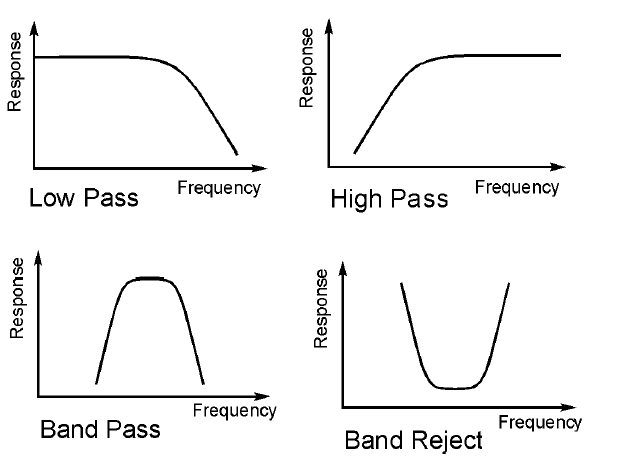
\includegraphics[scale=0.8]{figures/bproblemanalyse/filtertyper.png}
\caption{De fire filtertyper ses her \cite{2. semester kristian}\fxnote{Må man citere til en forelæsning?}}
\label{filtertyper}
\end{figure}

\subsection{Støj}
Støj er den uønskede del af et opsamlet signal, der ikke har nogen relation til det ønskede signal \fxnote{Må man citere til en forelæsning? - Hvis ja, så ved Nikoline, hvilken forelæsning det er}. Signaler, der er fordelt udover et frekvensspektrum, kan filtreres for støj vha. de tidligere beskrevne filtre. \cite{Devasahayam2000}
Støj kan inddeles i flere forskellige generelle typer, som typisk vil forekomme:

\begin{itemize}
\item Elektriske signaler: Dette er bl.a. 50 Hz støj, som er en frekvens fra elnettet. Denne 50 Hz frekvens kan gå ind og påvirke de biologiske signaler, der måles på. Hvis der er flere 50 Hz kilder, der interagerer, kan det give ekko ved eksempelvis 100 Hz og 150 Hz. Det er denne form for støj, der skal undgås, når signalet analyseres.
\item Ledninger: Kan fungere som antenner, der opfanger 50 Hz støj og andre former for støj. Problemet bliver større jo længere ledningen er. 
\item Magnetfelt: Kan komme i kontakt med ledningerne og derved inducere strømmen, der skaber støj i signalet. Jordens magnetfelt kan f.eks. påvirke ledningerne. For at mindske støjen kan ledningerne snoes / flettes sammen.
\end{itemize} 
% !TeX spellcheck = da_DK
\subsection{Komparator}\label{Komparatorafsnit}
En analog komparator er et kredsløb, der sammenligner en inputspænding eller -strøm med en eller flere referencespændinger eller -strømme. Rent teknisk gøres dette ved, at komparatoren inverterer inputsignalet $\pm 180^{\circ} V_{-}$, imens referencesignalet ikke inverteres $(V_{+})$. Hvis inputsignalet passer med en eller flere af referenceværdierne, vil de tilknyttede komponenter aktiveres. Den simpleste komparator er en operationsforstærker uden modkobling. \cite{webster2009} \\
Komparatorens output går fra en mætningsgrænse til en anden, når det negative input af operationsforstærkeren passerer igennem 0 V. Dette betyder, at ved et inputsignal på mere end tærskelniveauet vil outputsignalet opnå negativ mætningsgrad. Omvendt ved et inputsignal, som er lavere end tærskelniveauet, vil outputsignalet opnå positiv mætningsgrad. \cite{webster2009} 

%Det kan være fordelagtig at placere modstanden R1 ved inputsignalet, som det kan ses på \figref{komparator}, da dette minimerer overstyringen\fxnote{Et bedre ord end overstyring} af operationsforstærkeren.  Når inputtet, ved en simpel komparator, når tærskelniveauet og der forekommer støj på inputtet, kan outputsignalet svinge kraftigt. Dette kan imidlertid undgås ved at tilføje to modstande, R2 og R3. \cite{webster2009}

% !TeX spellcheck = da_DK
\subsection{ADC og konvertering til computeren}
Når der foretages målinger på kroppens signaler er output et analogt signal, som er kontinuert i tid og amplitude. Ved behandling af det analoge signal anvendes digital processering, hvilket betyder, at det analoge signal skal konverteres til et digital signal vha. en ADV (Analog-to-Digital-Converter). Det digitale signal er diskret i tid og amplitude, så det analoge signal kvantificeres under konverteringen \cite{Webster2009}. Konverteringsprocessen består af to dele, som er sampling og kvantisering \cite{Zouridakis2003}.  

Sampling er processen, hvor diskretisering i tidsdomænet finder sted, dvs. tidsdomænet i det kontinuerte signal konverteres til et diskret signal. Samplingsfrekvensen er den hyppighed hvormed signalet måles og hvis der ikke vælges en passende samplingsfrekvens, kan information fra det originale signal gå tabt. Ifølge Nyquists teorem er en hensigtsmæssig samplingsfrekvens således, at samplingsfrekvensen skal være mindst det dobbelte af frekvensen i det originale signal. \cite{Zouridakis2003} Det anbefales dog i praksis at sample med en samplingsfrekvens, der er ti gange frekvensen af det originale signal \fx{kilde??}. En for lav samplingsrate kan medføre, at kurven fra det rekonstruerede signal ligger forskudt ift. det originale signal, hvilket kaldes alias. \cite{Zouridakis2003}
 
Diskretisering af amplituden betegnes som kvantisering. De enkelte samples har en amplitudeværdi og ved kvantisering inddeles denne analoge værdi i trin. I modsætning til samling sker der en approksimering i det rekonstruerede signal, da værdierne mellem to trin repræsenteres af samme digitale værdi. \cite{Zouridakis2003} Antallet af amplitudeniveauer, der er tilgængelige til at repræsentere det analoge signal, determineres af antal bits. F.eks. en ADC med en opløsning på 12-bit inddeles i 4096 niveauer, da $2^12$=4096. \cite{Konrad2006} Det mindste amplitudeniveau ADC'en kan opnå kaldes LSB (Least Significant Bit) og bestemmes ved følgende ligning \fxnote{kilde?? - mine noter}: $LSB = \frac{FSR}{(2n-1)} = \frac{FSR}/{2^n}$, hvor FSR er "full scale voltage range" (arbejdsområdet), n er antal bits, $2^n$ er antal værdier og $2^n$-1 er antal intervaller. 

Ved forstærkning er det essentielt at være opmærksom på ADC'ens \fxnote{kan man skrive det?} arbejdsområde. F.eks. hvis signalet er højere eller mindre end ADC'ens arbejdsområde, vil signalet blive klippet. \fxnote{problemer igen med at finde nogle kilder til det} 
 
\clearpage
% !TeX spellcheck = da_DK
\section{Problemafgrænsning}
Apopleksi er en sygdom, der har stor indflydelse på blodtilførslen til encephalon. Hvis tilstrømningen af blod er nedsat, kan der opstå både motoriske og sensoriske skader hos patienten, hvilket kan komme til udtryk som balanceproblemer. Balancen er vigtig for at kunne fungere i dagligdagen, da den sikrer at man holder kroppen oprejst og muliggør bevægelse uden fald. \cite{Nichols1997} Apopleksipatienter med balanceproblemer oplever en begrænsning i deres dagligdag, da de er afhængige af hjælp til daglige gøremål, som de før sygdommen selv kunne udføre. De oplever det som et brud på deres tidligere liv, hvilket påvirker deres identitet og livskvalitet. \cite{Sundhedsstyrelsen2010}

For at begrænse de fysiske, og dermed også de personlige, følger mest muligt, er det essentielt at rehabiliteringen påbegyndes hurtigt efter apopleksitilfældet. Rehabilitering omfatter både genoptræning af fysiske funktioner, herunder balancefunktionen, men også tilpasning til miljø og styrkelse af sociale kompetencer.\fxnote{Ingen kilde på dette i afsnittet..} Indenfor rehabilitering af balance tilbydes forskellige metoder, såsom... \fxnote{ex. 2 metoder fra nuværende metoder} En anden mulighed ift. rehabilitering af balancen er biofeedback. Studier viser positive resultater med biomekanisk biofeedback, hvor der måles på kroppens generelle motoriske egenskaber. \cite{Giggins2013} For at biofeedback er en mulighed, er det en forudsætning, at patientens kognitive evner er tilstrækkelige til at kunne blive instrueret og kunne huske de indlærte øvelser fra gang til gang. Derudover er der visse krav til de neurologiske og motoriske evner \fxnote{de krav de opstiller i afsnit om biofeedback til patienten kan komme ind her, så det bliver mere specifikt}. \cite{Middaugh1989}

Det er derfor interessant at undersøge, hvordan der kan udvikles et system baseret på biofeedback, der kan hjælpe patienter med at genoptræne deres balance. Det er relevant at undersøge, om der kan designes et system, som i højere grad tillader patienterne at bidrage til deres egen rehabilitering. Det er muligt, at dette kan begrænse nogle af patienternes personlige følger, da kontakten med sundhedspersonale i forbindelse med rehabiliteringen evt. kan begrænses, hvormed det normale hverdagsliv hurtigere kan genoptages. \fxnote{Jeg her mest bare forkortet problemafgrænsningen, så der skal muligvis tilføjes enkelte linjer, som der er blevet skrevet til efter Erikas rettelser for at spore os helt ind på problemet}

\section{Problemformulering}
Hvordan designes et biofeedback system således, at det hjælper apopleksipatienter under rehabilitering af balancen?


%Apopleksi er den tredje største dødsårsag i Danmark \cite{Hjernesagen2015a}. 
%Af alle tilfælde af apopleksi er den iskæmiske langt den hyppigste med 80-85\% af tilfældene, imens den hæmoragiske udgør 10-15\%.
%Sygdommen har stor indvirkning på blodtilførslen til encephalon, som er det område af hjernen, der bla. rummer cerebrum. I cerebrum sker behandlingen af bla. sensoriske signaler, tanker og følelser. Når blodtilførslen til encephalon, og dermed også cerebrum, er nedsat, vil der kunne opstå både motoriske og sensoriske skader hos patienten.
%Når en patient med formodet apopleksi bliver indlagt, er det vigtigt, at lægen laver en grundig undersøgelse af de sensoriske og motoriske evner. Herefter foretages videre undersøgelser, eksempelvis CT- eller MR-scanning, afhængigt af den givne situation. \cite{Sundhedsstyrelsen2009} Det er vigtigt, at behandlingen igangsættes hurtigst muligt for at begrænse følgevirkningerne\cite{Soenderborg2013}. Der findes flere forskellige behandlingsmetoder. Ved iskæmi foregår behandlingen f.eks. med blodfortyndende medicin, en såkaldt trombolysebehandling, der har til formål at opløse blodproppen \cite{Hjernesagen2015b}. \fxnote{Mangler vi ikke noget om behandlingen af hæmoragi??}
%Apopleksi kan medføre sensoriske og motoriske skader. Disse skader kan have stor indvirkning på patientens liv efter sygdomsforløbet og en række psykiske konsekvenser og nedsat livskvalitet, bla. pga. sygdommens pludselige opståen. \cite{Muus2008}
%To eksempler på følger er balanceproblemer og neglekt. Balancen er vigtig for at kunne fungere i dagligdagen, da den sikrer at man holder kroppen oprejst og muliggør bevægelse uden fald. \cite{Nichols1997} Apopleksipatienter kan f.eks. lide af "Pusher Syndrom", hvor de ubevidst læner sig væk fra deres raske side. Dette påvirker balancen og kan lede til ulykker. \cite{Karnath2003} Ved neglekt er patienten ikke bevidst om den ene kropshalvdel. Dette kan være enten et visuelt eller et kropsligt problem. \cite{Sundhed.dk}
%Fælles for de to typer af følger er, at de begrænser patienterne i deres dagligdag og gør dem afhængige af hjælp til mange ting, som de før sygdommen selv kunne udføre. Derfor opleves ofte alvorlige personlige følger, eksempelvis problemer med at opretholde personlige relationer. Derudover kan patienternes identitet og humør også påvirkes. \cite{Sundhedsstyrelsen2010}
%For at begrænse de fysiske - og dermed også de personlige - følger mest muligt, er det essentielt at rehabiliteringen påbegyndes hurtigt efter apopleksien. Rehabiliteringen omfatter både genoptræning af fysiske funktioner, men også tilpasning til miljø og styrkelse af sociale kompetencer.\fxnote{Ingen kilde på dette i afsnittet..} 
%I Danmark er rehabiliteringen organiseret således, at de forskellige aktører i sundhedssektoren arbejder sammen på tværs af hinanden. Dette tværfaglige samarbejde er vigtigt, da apopleksipatienterne er i kontakt med mange forskellige dele af systemet under deres sygdomsforløb. \cite{Sundhedsstyrelsen2010} 
%Der findes i dag flere forskellige metoder til rehabilitering, afhængig af hvilken type følger patienten er ramt af. Metoderne er baseret på forskellige principper, herunder bla. træning vha. lyd, mekanisk træning, spejling og sensorisk stimulation\cite{Bradt2010,Mehrholz2013,Thieme2012,Sundhedsstyrelsen2010}.
%En anden måde at rehabilitere på er vha. biofeedback. Ved biofeedback måles på biologiske signaler, der relaterer til det område eller den funktion, som skal rehabiliteres hos patienten. Disse data omsættes til et signal, der kan opfattes af patienten. \cite{Giggins2013} Der skelnes mellem fysiologisk- og biomekanisk biofeedback\cite{Giggins2013}. Ved fysiologisk biofeedback måles der på kroppens systemer, herunder muskelaktivitet, hjerterytme og respiration. Ved biomekanisk biofeedback måles der på kroppens generelle motoriske egenskaber, eksempelvis hvordan kroppen bevæger sig. Studier har generelt vist positive resultater for biomekanisk biofeedback ift. rehabilitering af balanceproblemer. \cite{Giggins2013}
%For at biofeedback er en mulighed, er det en forudsætning, at patientens kognitive evner er tilstrækkelige til at kunne blive instrueret og kunne huske de indlærte øvelser fra gang til gang. Derudover er der visse krav til de neurologiske og motoriske evner. \cite{Middaugh1989}

%Både når der ses på de samfundsmæssige og personlige omkostninger, er apopleksi en krævende sygdom. Dels fordi sygdomsforløbet foregår i flere forskellige dele af sundhedssystemet og er den sygdom, der kræver flest plejedøgn. Derudover medfører sygdommen alvorlige fysiologiske og mentale følger.

%Det er derfor interessant at undersøge hvordan der kan udvikles et system baseret på biofeedback, der kan hjælpe patienter med at genoptræne deres balance. Det er relevant at undersøge om der kan designes et system, som i højere grad tillader patienterne at bidrage til deres egen rehabilitering. Det er muligt, at dette kan begrænse nogle af patienternes personlige følger, da kontakten med sundhedspersonale i forbindelse med rehabiliteringen evt. kan begrænses, hvormed det normale hverdagsliv hurtigere kan genoptages. 

%Man kan derfor undersøge muligheden for at begrænse både de samfundsmæssige og personlige omkostninger for patienter med balanceproblemer vha. et system baseret på biofeedback. Hvis der kan udvikles et system, der i højere grad tillader patienten at genoptræne sin balance selv, ved at gøre vedkommende opmærksom på eventuel hældning til siden, vil dette muligvis kunne begrænse patientens behov for at være i kontakt med sundhedspersonale, hvormed en normal dagligdag også hurtigere kan påbegyndes igen.  

\chapter{Problemløsning}
% !TeX spellcheck = da_DK
\section{Systembeskrivelse}  

\subsection{Formål og anvendelse}
Systemet har til formål at gøre apopleksipatienter opmærksomme på, hvornår de mister balancen \fxnote{reference til problemafgrænsningen}. Systemet skal derfor kunne registrere, hvis patienten er i risiko for at falde og derved udsende et signal så patienterne har mulighed for at rette sig op igen. Selve systemet skal anvendes så patienterne er mere selvstændige i rehabiliteringsprocessen med henblik på at opnå en bedre balance. 

Det er på baggrund af afsnit.. valgt at hældningen på patienten skal opfanges via en sensor som er placeret på patienten. Systemet skal give visuelt feedback i form af to dioder, når patienten hælder til enten højre eller venstre. Når patienten hælder XX til den ene side indikeres det af en gul diode, hvis patienten hælder yderligere, hvilket svarer til en hældning på XX lyser en rød diode. Derudover anvendes sensorisk feedback via vibration som advarer patienten ved den gule diode og stiger i takt med at patienten hælder mere og mere.  
%Ud fra problemanalysen fremgår det, at ældre over 65 år i højere grad får apopleksi, hvortil balanceproblemer er en hyppig gene. Derudover har apopleksipatienter ofte kognitive problemer. Apopleksipatienter har et ønske om at være selvstændige og uafhængige. 

%Systemet skal opfange, hvis patienten er ude af balance og være nemt anvendeligt, da det skal bruges til selvtræning af balancen i hjemmet - altså implementeres i fase 4, som bliver omtalt på side \pageref{Faser}. For at systemet kan anvendes af målgruppen, skal det være brugervenligt - dvs. let at påsætte, ikke veje for meget samt signalerne skal være let forståelige. Målgruppen giver yderligere begrænsninger ift. feedback, da både hørelsen, synet eller kroppens følelser kan være svækket. Derudover skal systemet kunne give et digitalt output, som er muligt at behandle.

\subsection{Systemets brugere}
Systemet udvikles med henblik på selvtræning af balance i rehabiliteringsfasen. Derfor er systemets primære bruger patienten selv. Jævnfør afsnit (med apopleksipatienters alder) ses det at majoriteten af apopleksipatienter er over 65 år. Systemet skal være let anvendeligt så det kan anvendes af denne ældre demografi. Fagkyndigt personale, såsom fysioterapeuter og læger, skal kunne følge med i udviklingen som patienten gennemgår. Det skal derfor være muligt for disse også at benytte systemet. Dette gøres ved at systemet både har et analogt og digitalt output. Hvor det digitale henvender sig mere til et fagkyndigt personale.

\subsection{Anvendelse}
Systemet designes til at patienten under anvendelsen skal være stående på en tegnet linje med den ene fods tæer mod den anden fods hæl\fxnote{måske et billede vi tager som vil illustrere dette}. Denne position er valgt for at udfordre patientens balance ved at fordele kropsvægten anderledes ift. den normale kropsstilling omtalt på side \pageref{BalanceAfsnit}. Patienten påsætter selv systemet øverst på sternum og udfører herefter en kort prøvetest for at kende til de givne feedbackparametre. Under prøvetesten svajer patienten langsomt fra side til side. Hvis vedkommende hælder over xx grader, vil en gul diode lyse og vibrationen vil begynde. Hvis patienten svajer yderligere og hælder med over xx grader vil en rød diode lyse. Vibrationen vil styrkes i takt med overgangen fra den gule til den røde diode. Efter testøvelsen udføres selve træningsøvelsen. Her indtages udgangspositionen på linjen og øjnene lukkes. Dette gøres for at udelukke den visuelle sans, hvilket gør det sværere for patienten at opretholde balancen. Patienten skal forsøge at holde balancen så længe som muligt uden at bevæge sig ud i risikozonerne, der vil blive markeret ved vibration. Træningsøvelsen gentages efter behov. \\
Ved at tage flere målinger igennem rehabiliteringsforløbet vil det forventes at der sker en fremgang ift. tiden hvori balancen kan opretholdes uden at patienten bevæge sig ud i risikozonerne. 

\subsection{Optagelse af signal fra accelerometer}
Acceleorometeret skal give et elektrisk signal ud fra den position som anvendes i forsøget \fxnote{Vi skal vurdere hvor signalet kommer fra om det x,y,z aksen.}. Accelerometeret opfanger de signaler som udsendes fra sensoren som er placeret anteriort på patientens brystkasse. Signalet afhænger af, hvor langt patienten har flyttet sig. 

............ HER MANGLER NOGET INFORMATION..........................

Ledningerne snoes for at kontrollere samt mindske støjen. Derudover sættes ledninger fast med tape på patienten, så vidt det er muligt. For at undgå unødvendigt støj foretages forsøget væk fra andet elektronik.  %\ref{reference til støj afsnittet}



\subsection{Analogt output}
Det analoge output skal kunne henvende sig til patienten, dette sker ved lysdioder og vibration. Lysdioderne skal lyse gult ved 'usikkerhed' og slukke hvis patienten enten er rettet op igen eller bevæger sig ud i riskozonen, hvorefter en ny diode skal lyse rødt. Vibrationerne igangsættes ved 'usikkerhed' og skal stoppe hvis patienten retter sig op eller stige i styrke, hvis patienten kommer ud i risikozonen. 

\subsection{Digitalt output}
Det digitale skal kunne anvendes af sundhedspersonale til at vurdere om patienten gør fremskridt, dette indebærer at informationerne for patienten kan gemmes og sammenlignes på en computer. 


\subsection{Systemets opbygning}
Systemets opbygning fremgår af \figref{kravblok}.

\begin{figure}[H]
	\centering
	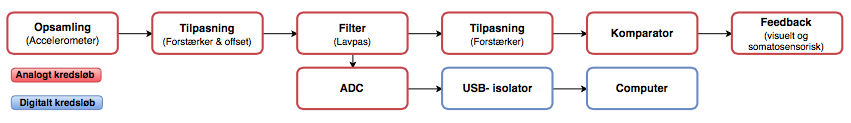
\includegraphics[scale=0.62]{figures/cProblemloesning/blokdiagram1.png}
	\caption{Figuren viser de blokke/elementer som systemet skal indeholde}
	\label{kravblok}
\end{figure}

Signalerne fra accelerometeret skal forstrækes, herefter støj skal filteres fra for at dæmpe uønskede frekvenser. Herefter forstærkes signalet med en variabel forstærkningen, da signalet kun er forstærket lidt. Signalet forstærkes til maksimalt 3V. Dette gøres ved en operationsforstærker \fxnote{inverteret eller ikke-inverteret} Det analoge signal ensrettet via. \fxnote{helbølgeensretter eller halvbølgeensretter}, hvor efter der benyttes en integrator til at lave en lineær linje. Ud fra denne linje gives en advarsel via feedback. Det digitale signal skal konverteres fra analogt til digitalt, hvilket gøres ved en ADC.  Herefter anvendes en USB-isolator for patientsikkerhed. Computeren skal fremvise en graf når NIDAQ er tilsluttet. 

\subsection{Kravspecifikationer}
Til vurdering af tolerance er der udført et pilotforsøg, dette er udført med henblik på at kunne beregne forstærkning, filtrering og integrering af signalet. 

\subsubsection{Det samlede system}
Det analoge output sammenligninger inputtet som kommer fra accelerometeret og outputtet i form af 2 dioder og stigning i vibration. Aktivering af bestemte dioder skal afspejle inputsignalet således at et lille input aktiverer en gul diode og vibration, mens et større input aktiverer en rød diode og stigningen i vibration. 

\textbf{Krav:}
\begin{itemize}
\item Den gule diode skal lyse når patienten har bevæget sig XX og slukke hvis patienten retter sig op eller hælder yderligere.
\item Den røde diode skal lyse når patienten har bevæget sig XX og slukke, hvis patienten retter sig op.
\item Vibration skal igangsættes når patienten har bevæget sig XX og skal slukke, hvis patienten retter sig op eller stige, hvis patienten hælder yderligere.
\item Der skal være en sammenhæng mellem inputsignalets størrelse og antallet af dioder der lyser?
\item Signalet i systemet må ikke forstærkes til en værdi over 3V.
\end{itemize}

\subsection{Krav}
For at gøre anvendelse af samme system muligt til 4. Semester skal arbejdsområdet kunne benyttes sammen med et USB-baseret trådløst udviklingsværktøj eZ430-RF2500 fra Texas Instruments. Det er derfor nødvendigt, at designet stemmer overens med udviklingsværktøjet for at kunne sende og modtage data til og fra computeren. Udviklingsværktøjet indeholder hardware og software som evaluerer mikrokontrolleren MSP430F2274. For at hele vores system kan anvendes med udviklingsværktøjet, skal outputsignalet være 3V, eftersom mikrokontrolleren opererer med spændingsforsyning mellem 1,8V og 3,6V.

%\textbf{Tolerance:}
%\begin{itemize}
%\end{itemize}
%
%\subsubsection{Accelerometer}
%\textbf{Krav:}
%\begin{itemize}
%\end{itemize}
%
%\textbf{Tolerance:}
%\begin{itemize}
%end{itemize}
%
%\subsubsection{Instrumentering forstærker}
%\textbf{Krav:}
%\begin{itemize}
%\end{itemize}
%
%\textbf{Tolerance:}
%\begin{itemize}
%\end{itemize}
%
%\subsubsection{Filtre - opdeling i høj og lavpass?}
%\textbf{Krav:}
%\begin{itemize}
%\end{itemize}
%
%\textbf{Tolerance:}
%\begin{itemize}
%\end{itemize}

%\subsubsection{Forstærker med variabel forstærkning}

%\textbf{Krav:}
%\begin{itemize}
%\end{itemize}
%
%\textbf{Tolerance:}
%\begin{itemize}
%\end{itemize}
%
%\subsubsection{Ensretter}

%\textbf{Krav:}
%\begin{itemize}
%\end{itemize}
%
%\textbf{Tolerance:}
%begin{itemize}
%end{itemize}
%
%\subsubsection{Integrator}
%\textbf{Krav:}
%\begin{itemize}
%\end{itemize}
%
%\textbf{Tolerance:}
%\begin{itemize}
%\end{itemize}
%
%\subsubsection{Advarsel}
%\textbf{Krav:}
%\begin{itemize}
%\end{itemize}
%
%\textbf{Tolerance:}
%\begin{itemize}
%\end{itemize}
%
%\subsubsection{ADC}
%\textbf{Krav:}
%\begin{itemize}
%\end{itemize}
%
%\textbf{Tolerance:}
%\begin{itemize}
%\end{itemize}
%
%\subsubsection{USB-isolator}
%\textbf{Krav:}
%\begin{itemize}
%\end{itemize}
%
%\textbf{Tolerance:}
%\begin{itemize}
%\end{itemize}
%
%\subsubsection{Computer}
%\textbf{Krav:}
%\begin{itemize}
%\end{itemize}
%
%\textbf{Tolerance:}
%\begin{itemize}
%\end{itemize}
%\begin{itemize}
%\item Systemet skal ved fald få dioder til at lyse samt give feedback i form af stigende vibration. 
%\item Systemet skal være non-invasiv - dvs. systemet ikke må påføre patienten smerte eller varig skade
%\item Systemet skal være brugervenligt
%\item Systemet skal forsynes med spænding fra 9V batteri
%\end{itemize}

%\subsubsection{Accelerometer}
%Accelerometeret skal detektere patientens kropshældning.

%\subsubsection{Filter}
%Når der anvendes et filter, skal det dæmpe uønskede frekvenser. Dvs. frekvenser der lavere eller højere ift. det signal fra accelerometeret, som man vil analysere på. Der skal udføres et pilotforsøg for at finde frem til det korrekte filter og valg af knækfrekvens. 

%\subsubsection{Signalerende lys}
%Når patienten er ude af balance skal en rød diode lyse, som signalering ift. patientens hældning. Der skal vha. et pilotforsøg detekteres, hvornår dioden skal lyse. Skal der evt. være 2 dioder, hvor den ene er et "advarende" signal og nr. to er "fare". 

%\subsubsection{Alarm/vibrationen}
%Alarmen/vibrationen skal anvendes i perioden, hvor patienten er ude af balance og stoppe igen, når der igen er oprettet balance. 
%(eller fungere som en alarm til dioderne - så når en diode lyser, skal alarmen gå)

%\subsubsection{ADC}
%Der anvendes en ADC i systemet, for at konvertere det analoge signal til digitalt. Det næste skridt er konverteringen til PC og det er derfor essentielt at have en ADC, der konverterer analogt signal til binære tal, som digitale systemet anvender. 
%{Her skal vi have valgt en samplingsfrekvens)

%\subsubsection{USB-isolater}
%USB-isolatoren sikre patientens sikkerhed. Her skal input- og outputspænding være ens.  

%\subsubsection{Til PC}
%Fremvisning af graf, så patienten og plejepersonale kan følge %rehabiliteringens udvikling. 

% !TeX spellcheck = da_DK
\section{Overordnede funktionelle krav til systemet}\label{FunkKrav}
\begin{itemize}
	\item Systemet skal være simpelt, så det kan anvendes af både apopleksipatienterne selv samt af fagkyndigt personale
	\item Systemet skal kunne måle kropshældning, samt angive hvilken retning hældningen sker mod. 
	\item Systemet skal kunne give visuel og somatosensorisk feedback ved forskellige hældningsgrader.
	\begin{itemize}
		\item Grøn diode: Skal lyse, når patienten ikke er ude i risikozonerne og informere patienten om at accelerometeret er placeret korrekt.  
		\item Gul diode: Skal lyse, når den første risikozone defineret i grader indtræffer og slukke, hvis patienten retter sig op.
		\item Rød diode: Skal lyse, når den anden risikozone defineret i grader indtræffer og slukke, hvis patienten retter sig op.
		\item Vibration: Skal aktiveres, når den første risikozone indtræffer og skal slukke, hvis patienten retter sig op. Hvis patienten hælder yderligere, skal vibrationshastigheden stige.
	\end{itemize}
	\item Systemet skal kunne skifte mellem to sværhedsgrader, hvilket vil sige, at systemet skal kunne skifte imellem to forskellige komparator blokke, som har tærskelværdier relateret til sværhedsgraden af den udførte øvelse.
	\item Systemet skal kunne give et digitalt outout, så fagkyndigt personale kan behandle og gemme patienternes data i et program.
\end{itemize}

% !TeX spellcheck = da_DK
\section{Pilotforsøg}\label{Sec:Pilotforsoeg}
Det er nødvendigt at kunne skelne det reelle signal fra støjkomponenter, før systemet kan designes. Signalet skal aktivere komponenter i slutningen af det analoge system og skal derfor være adskilt fra støj, der kan påvirke outputtet. For at undgå dette frafiltreres støjsignaler. Derudover er det nødvendigt at vide, hvilket outputsignal accelerometeret giver ift. den valgte hældningsgrad. Dette gøres ud fra sensitiviteten, der måles. Ud fra disse oplysninger er det muligt at kravspecificere de enkelte blokke i systemet.% Oplysningerne findes på baggrund af et pilotforsøg. 

\subsection{Formål med pilotforsøg}
\begin{enumerate}
\item Identificere de frekvenser, der udgør støj i outputsignalet fra accelerometeret.
%\item Udregner accelerometerets g-påvirkning ved $8^{\circ}$ og $13^{\circ}$.
\item Identificere maksimum og minimum outputsignal af accelerometeret.
\item Kontrollere om offset og sensitivitets værdierne fra databladet på accelerometeret stemmer overens med målt data.
\end{enumerate}

\subsection{Materialer}
\begin{itemize}
\item ADXL335 accelerometer.
\item To stk. $0.1\mu$F kondensatorer.
\item Ledninger.
\item Breadboard.
\item $5V$ fra spændingsforsyning.
\item NI USB-6009.
\item USB isolator USI-01.
\item Computer med ScopeLogger og MATLAB R2015a.
\item Hæftemasse.
\item Vinkel.
\item Vaterpas.
\item Termometer
\end{itemize}

\subsection{Metode}
Støjfrekvenserne i outputsignalet identificeres ved først at måle en baseline ved $0g$ dvs. uden hældning. Dette medfører at signalet kan analyseres uden nogen påvirkning på outputsignalet. Dernæst måles en påvirkningen ved $1$g, hvilket svarer til en hældning på $90^{\circ}$. Dette måles både til højre og venstre. Derved kan det sammenlignes, om der er støj ift. baseline. %Det samme gøres for de specificerede hældningsgrader, som er $8^{\circ}$ og $13^{\circ}$. 
For at simulere den påvirkning, accelerometeret udsættes for og identificere den mulige støj ved en rotation, roteres accelerometret i en langsom rotation fra $0^{\circ}$ til $90^{\circ}$ til både højre og venstre. Disse målinger vil identificere minimum og maksimum outputsignal, som accelerometeret kan afgive i dette tilfælde, samt kontrollere om offset og sensitivitet informationerne fra accelerometerets datablad stemmer overens med det målte data. \\
Inden, under og efter forsøget måles temperaturen i lokalet, da denne kan have en effekt på accelerometerets sensitivitet. \cite{Devices2009}

\subsection{Forsøgsopsætning på breadboard}
\textbf{Opsætning}\\
Der ses et billede af forsøgsopsætningen på breadboardet på \figref{pforsoeg1}.
\begin{itemize}
\item Accelerometeret tilkobles breadboardet.
\item To kondensatorer på $0.1\mu$F tilkobles breadboardet. Kondensatorererne er valgt på baggrund af databladet for acceleorometeret ift. power supply decoupling og båndbredde.\fxnote{Den som sidder på pin $1$ og $2$ i accelerometeret fjerner støj fra strømforsygningen, mens kondensatoren fra pin $3$ giver en båndbredde på $50Hz$.}
\item Accelerometeret tilnyttes en forsyningsspænding på $7V$ - en regulator sikrer at det kun forsynes med en spænding indenfor dets arbejdsområde.
\item Outputtet fra systemet sendes igennem en ADC af typen NI USB-6009.
\item Signalet fra NI USB-6009 sendes igennem en USB-isolator af typen USI-01.
\item Outputsignalet fra USI-01 sendes ind i computeren, hvor det optages med ScopeLogger og behandles i MATLAB R2015a.
\end{itemize}

\begin{figure}[H]
	\centering
	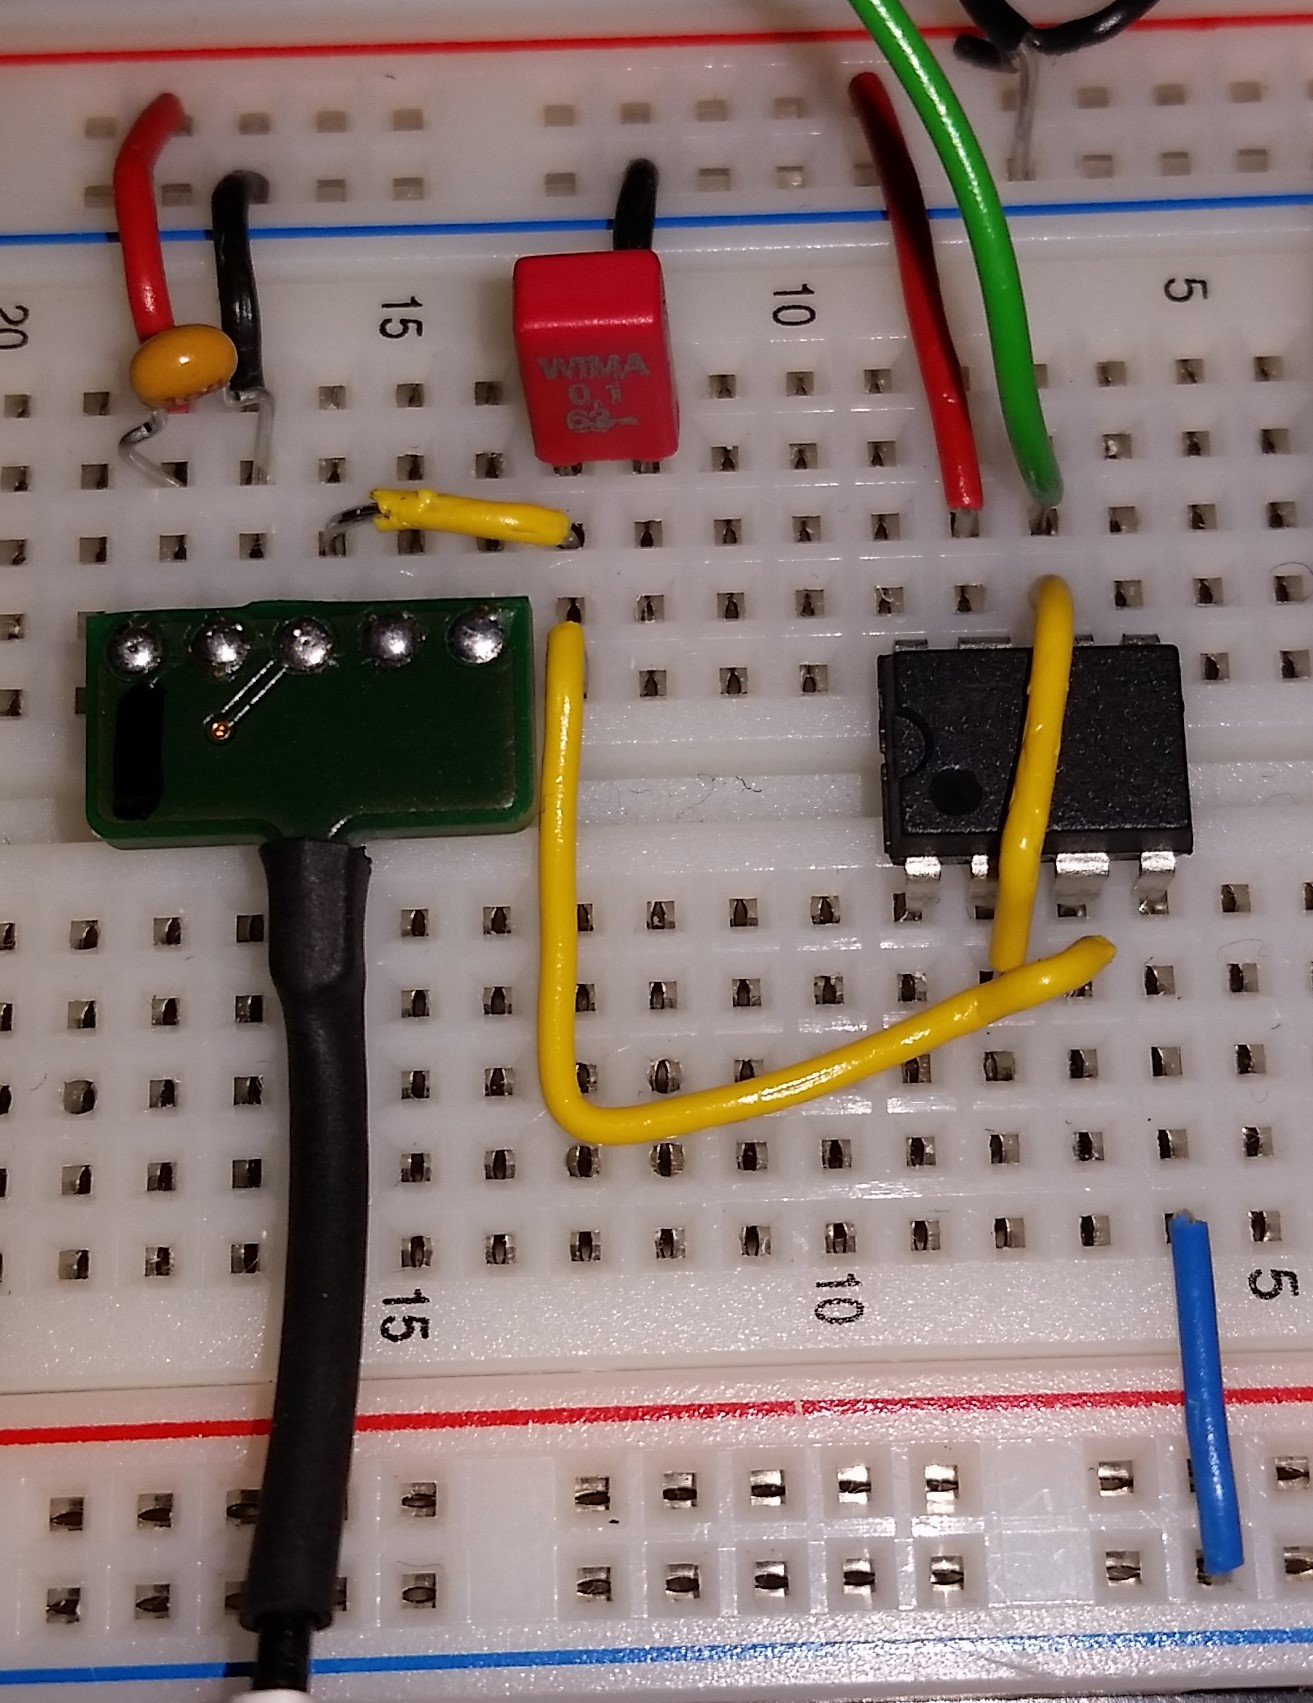
\includegraphics[scale=0.15]{figures/cProblemloesning/PF2.jpg}
	\caption{På billedet ses opsætningen på breadboardet. De røde ledninger symboliserer inputtet fra den $5V$ spændingsforsyning. De sorte ledninger leder til ground. Den gule ledning fungerer som en leder for outputtet fra accelerometerets pågældende akse (kan skiftes imellem række $15$, $16$ og $17$ alt efter hvilken akse, der skal måles på). Den grønne ledning symboliserer outputtet fra kredsløbet, som sendes til NI USB-6009.}
	\label{pforsoeg1}
\end{figure}

\subsection{Fremgangsmåde}
\subsubsection{Forsøgets udførelse}
Hele pilotforsøgets opsætning ses på \figref{pforsoeg2}. \\
For at måle $0g$ påvirkning på accelerometerets x-akse, lægges det fladt ned på et plant bord, som er tjekket med et vaterpas. Målingen gøres over tre omgange i $30$ sekunder. Herefter holdes accelerometeret fast på en vinkel, hvor ledningerne påsættes med hæftemasse. Accelerometeret sættes så der igen måles på x-aksen, når der sker en rotation til højre og venstre. Vinklen sættes således, at der måles $1g$ påvirkning i positiv retning og negativ retning, hvilket svarer til $\pm90^{\circ}$ fra accelerometerets nulpunkt. \\
Dette giver tre baselines for hver g påvirkning, som opsamles og gemmes i ScopeLogger. %Herudover måles en baseline for g påvirkningen af accelerometeret ved $8^{\circ}$ og $13^{\circ}$. Dette gøres ved at holde accelerometeret i 30 sekunder på $8^{\circ}$ og $13^{\circ}$ henholdsvis til højre og venstre. Herved fås 4 baselines, som optages og gemmes i ScopeLogger. 
Til sidst måles g påvirkningen af accelerometeret under rotation fra $0^{\circ}$ til $\pm$ $90^{\circ}$ for både højre og venstre. Her måles $10$ sekunders baseline inden og efter rotationen, som varer $10$ sekunder og foretages langsomt og kontrolleret. Disse to målinger optages og gemmes ligeså i ScopeLogger. \\
\subsubsection{Behandling af data}
Efter udførelse af forsøget vil alt data blive behandlet i MATLAB R2015a, hvor der beregnes en gennemsnitsværdi for henholdsvis de tre baselines målt ved $0g$ påvirkning samt $1g$ påvirkning i positiv retning og negativ retning. Der foretages desuden en Fast Fourier Transformation (FFT) på de ni målinger (tre målinger ved hver g påvirkning). FFT foretages for at få en grafisk repræsentation af det målte signal i frekvensdomænet. Baseline optages for at se hvilken påvirkning omgivelserne har på signalet, da der ikke er nogen bevægelse på disse.

\begin{figure}[H]
	\centering
	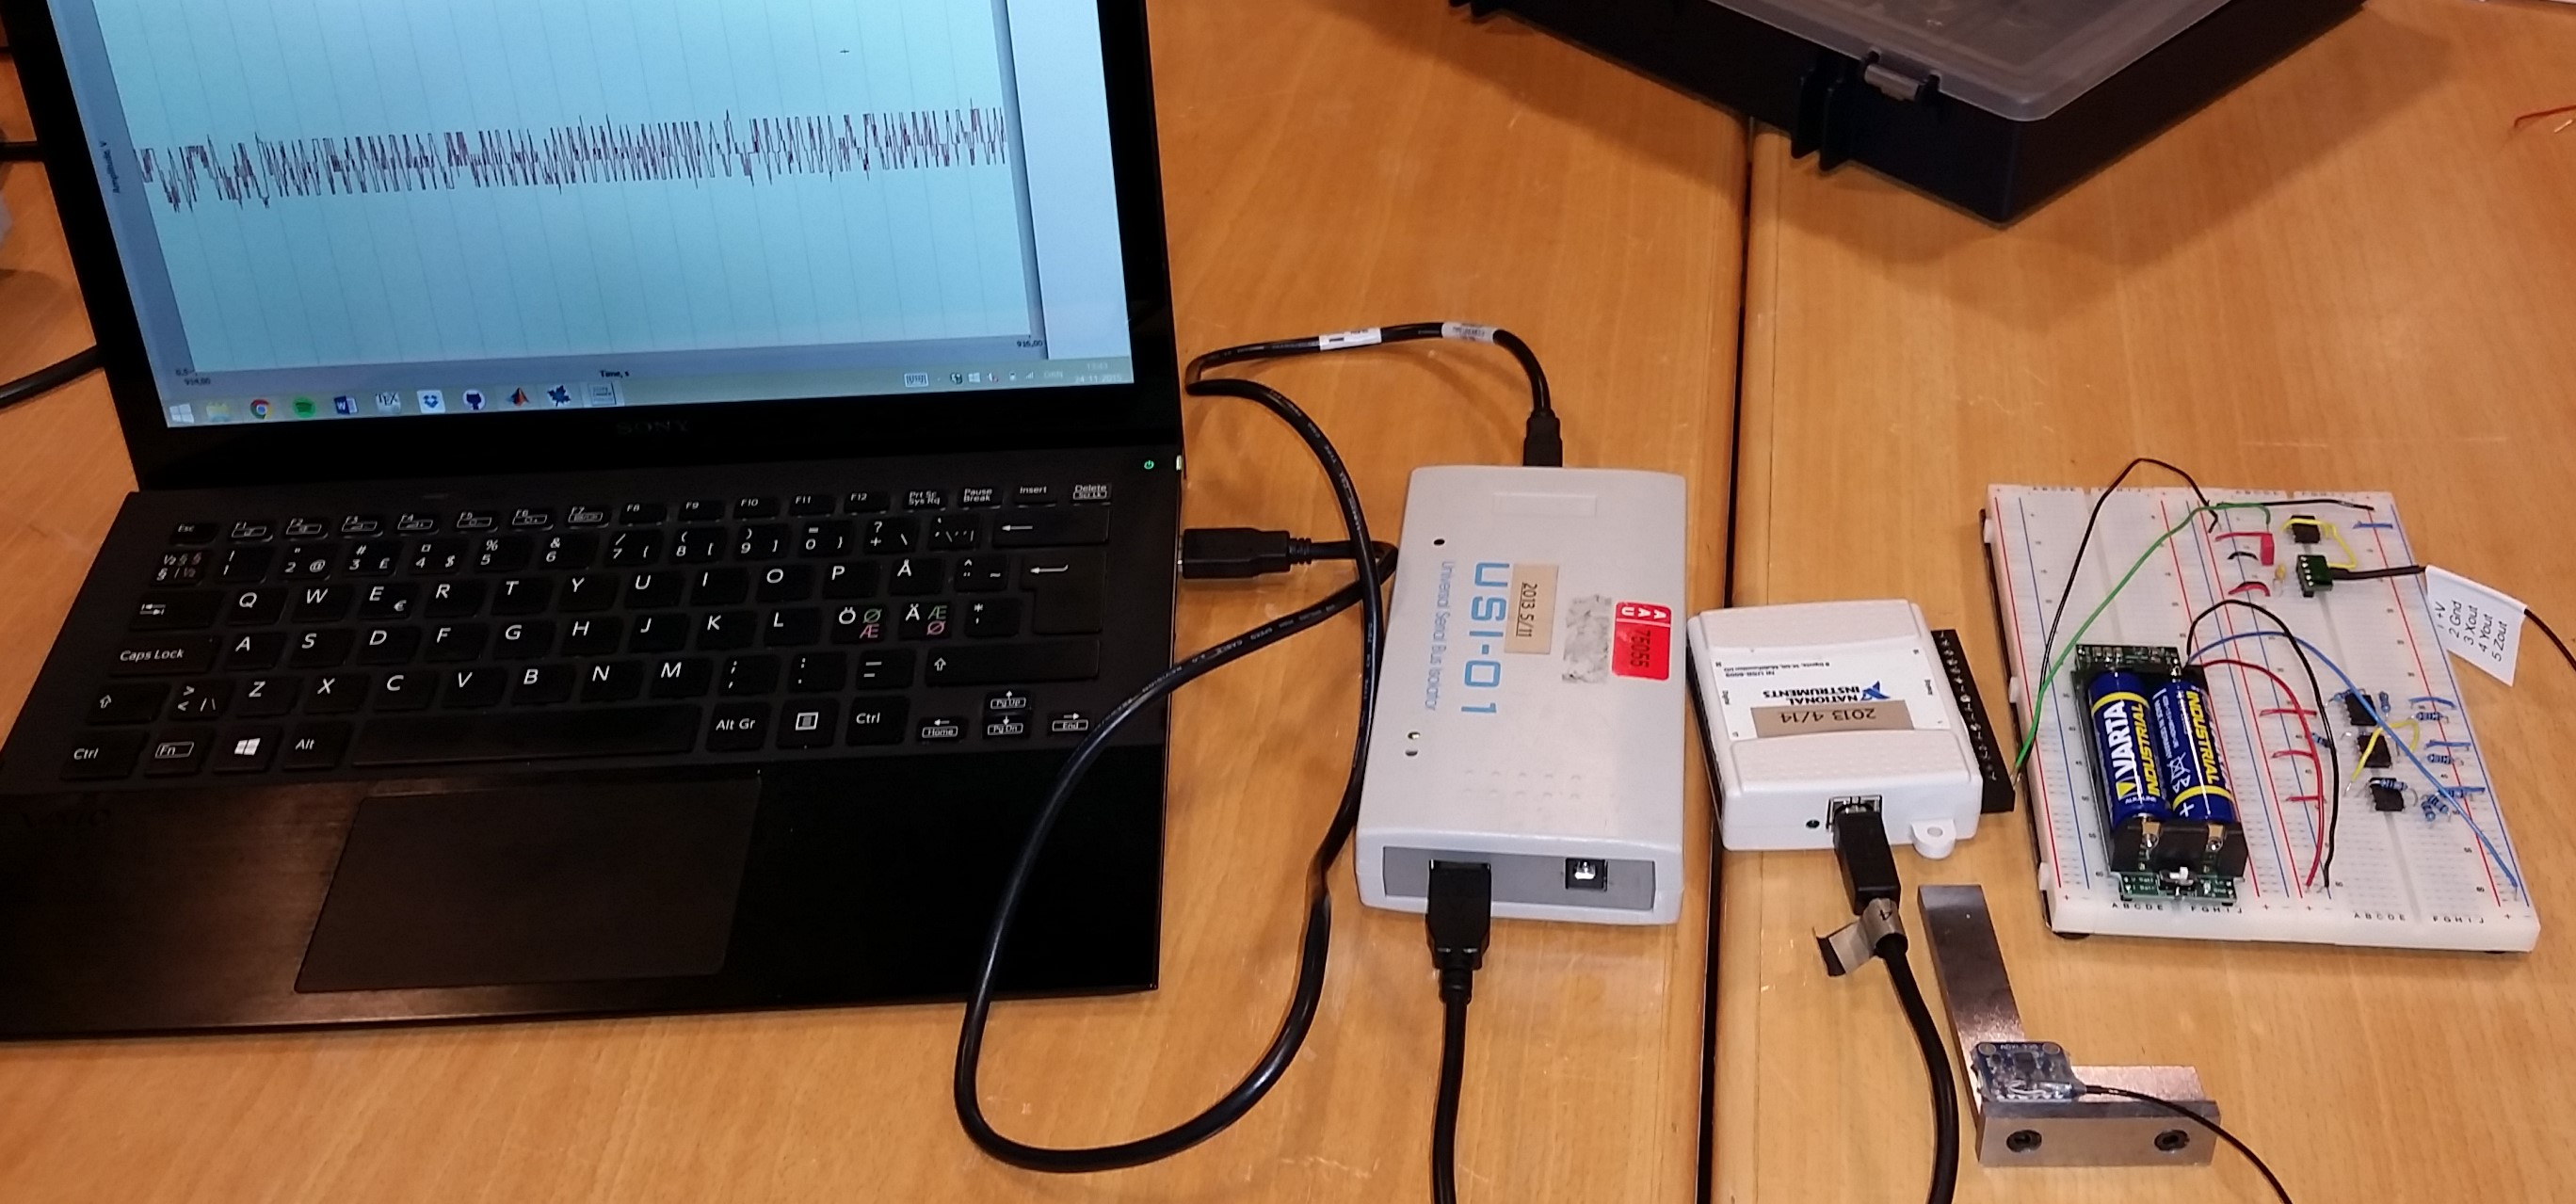
\includegraphics[scale=0.14]{figures/cProblemloesning/Pilotforsoeg1_2.jpg}
	\caption{På billedet ses (fra venstre til højre) den 5V spændingsforsyning, som leder strømmen til og fra ground fra breadboardet. Fra breadboardet sendes outputtet videre til ADC'en(NI USB-6009). Herefter ledes signalet igennem USB-isolatoren(USI-01) og til sidst ind i computeren, hvor det optages i ScopeLogger. Over breadboardet i midten på billedet ses vaterpasset. Forrest i midten på billedet ses accelerometret fastgjort på vinklen.}
	\label{pforsoeg2}
\end{figure}

\subsection{Resultater}\label{Sec_Pilot_Data}
I dette afsnit vil der grafisk blive vist, hvordan accelerometerets output ændrer sig ift. g påvirkning. På \figref{Fig:Pilot_Tid} ses accelerometerets output i tidsdomænet. Der udføres herefter en FFT på de tre målinger for hver baseline, hvilket giver ni grafiske skiltninger af, hvorledes accelerometerets egne frekvenser adskiller sig fra støjfrekvenser.

\begin{figure}[H]
	\centering
	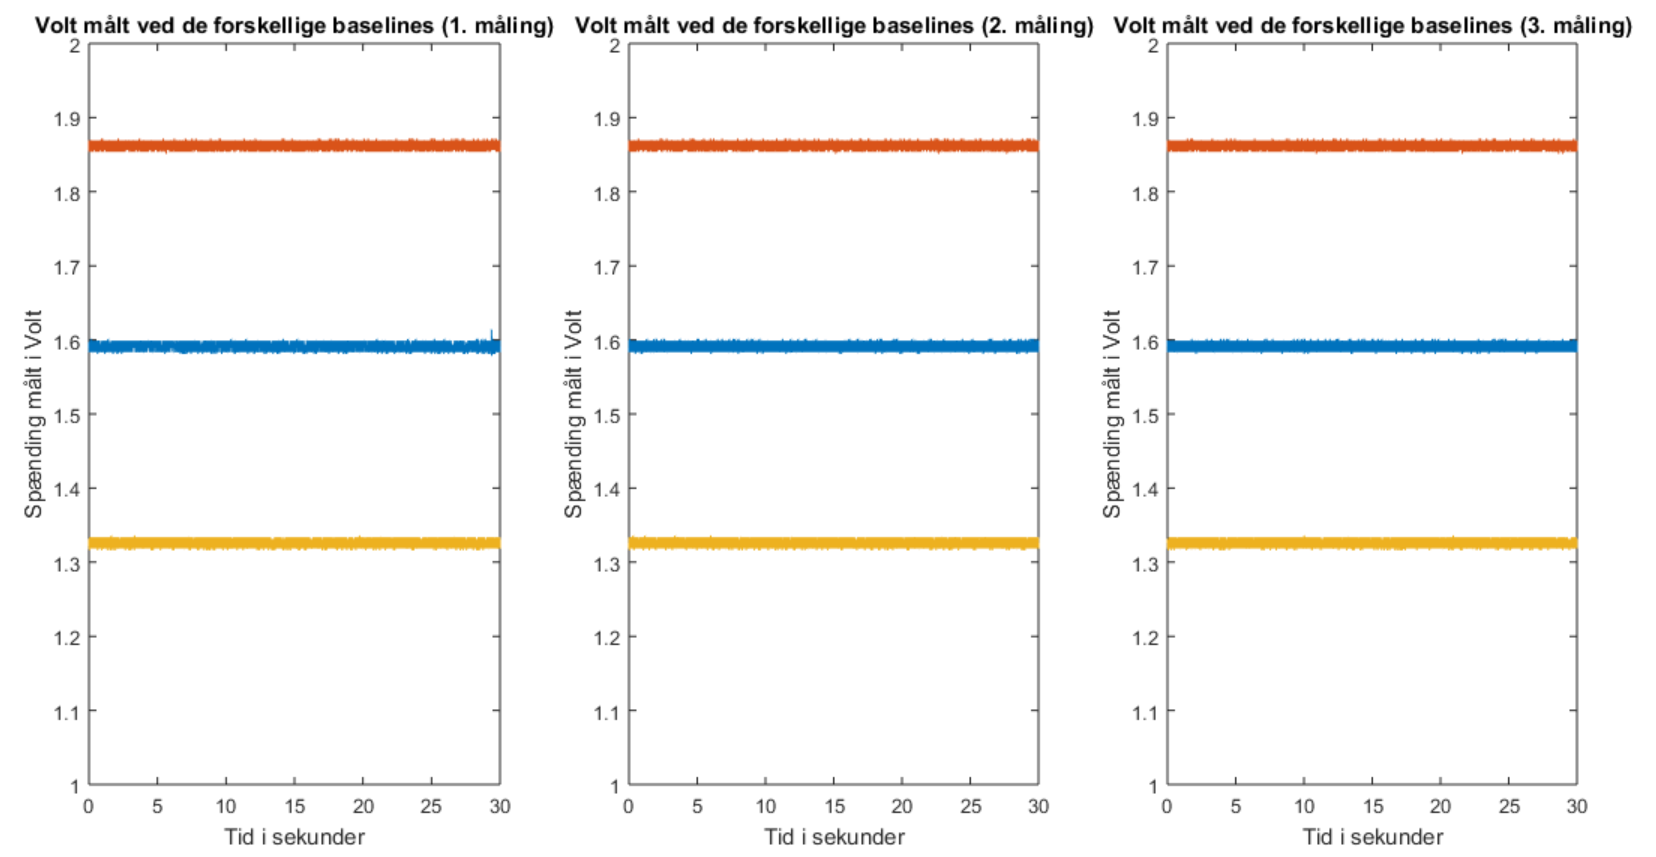
\includegraphics[scale=0.45]{figures/cProblemloesning/Pilotforsoeg_Tid.png}
	\caption{På graferne ses henholdsvis første, anden og tredje måling for hver g påvirkning af accelerometret. Den røde graf repræsenterer outputtet målt ved $1g$ påvirkning i positiv retning. Den blå graf repræsenterer outputtet målt ved $0g$ påvirkning. Den gule graf repræsenterer outputtet målt ved $1g$ påvirkning i negativ retning.}
	\label{Fig:Pilot_Tid}
\end{figure}

Offsettet for accelerometerets x-akse udregnes ved at tage den målte gennemsnitsværdi ved $0$g for alle tre målinger og yderligere tage gennemsnittet af disse. De tre målinger ses som de blå grafer på \figref{Fig:Pilot_Tid}. Udregningen ses på \ref{Mean_tid_0g}:
\begin{equation}\label{Mean_tid_0g}
\text{Offset} = \frac{1.5911 + 1.5916 + 1.5916}{3} = 1.5915
\end{equation}
\noindent Offsettet burde ifølge databladet for accelerometret være halvdelen af spændingsforsyningen, som i dette tilfælde leder en spænding på $3.3V$. \cite{Devices2009} Derfor burde offsettet være $1.65V$. Afvigelsen kan derved udregnes:
\begin{equation}
\text{Afvigelse for offset} = \dfrac{1.5915 - 1.65}{1.65} \cdot 100 = -3.5481\% \approx 3.5\%
\end{equation}

\noindent Herefter kan sensitiviteten for accelerometeret udregnes. Dette gøres ved først at udregne en gennemsnitsværdi for $1g$ påvirkning i henholdsvis positiv og negativ retning. Værdierne for $1$g påvirkning i positiv retning er angivet som de røde grafer på \figref{Fig:Pilot_Tid}, imens de i negativ retning er angivet som de gule grafer. Efter udregningen af gennemsnittet trækkes den udregnede offset værdi fra.
\begin{align}
	\text{Gennemsnit 1g positiv retning} = \frac{1.8627 + 1.8627 + 1.8626}{3} = 1.8627 \\
	\text{Gennemsnit 1g negativ retning} = \frac{1.3254 + 1.3255 + 1.3254}{3} = 1.3254 \\
	\text{Sensitivitet positiv retning} = 1.8627 - 1.5915 = 0.2712 \\
	\text{Sensitivitet negativ retning} = 1.3254 - 1.5915 = -0.2660
\end{align}
\noindent Da der findes en lineær sammenhæng imellem g påvirkning og outputtet burde sensitiviteten for accelerometret med en spændingsforsyning på $3.3V$ være $330mV/g$. Der kan derved udregnes afvigelse for både negativ og positiv retning:
\begin{align}
	\text{Afvigelse for sensitivitet i positiv retning} = \dfrac{0.2712 - 0.330}{0.330} = -17.8182\% \approx 17.8\% \\
	\text{Afvigelse for sensitivitet i negativ retning} = \dfrac{0.2660 - 0.330}{0.330} = -19.3940\% \approx 19.4\%
\end{align}

På \figref{Fig:Pilot_FFT0}, \figref{Fig:Pilot_FFTN} samt \figref{Fig:Pilot_FFTP} ses en FFT af det målte data for statisk acceleration.
\begin{figure}[H]
	\centering
	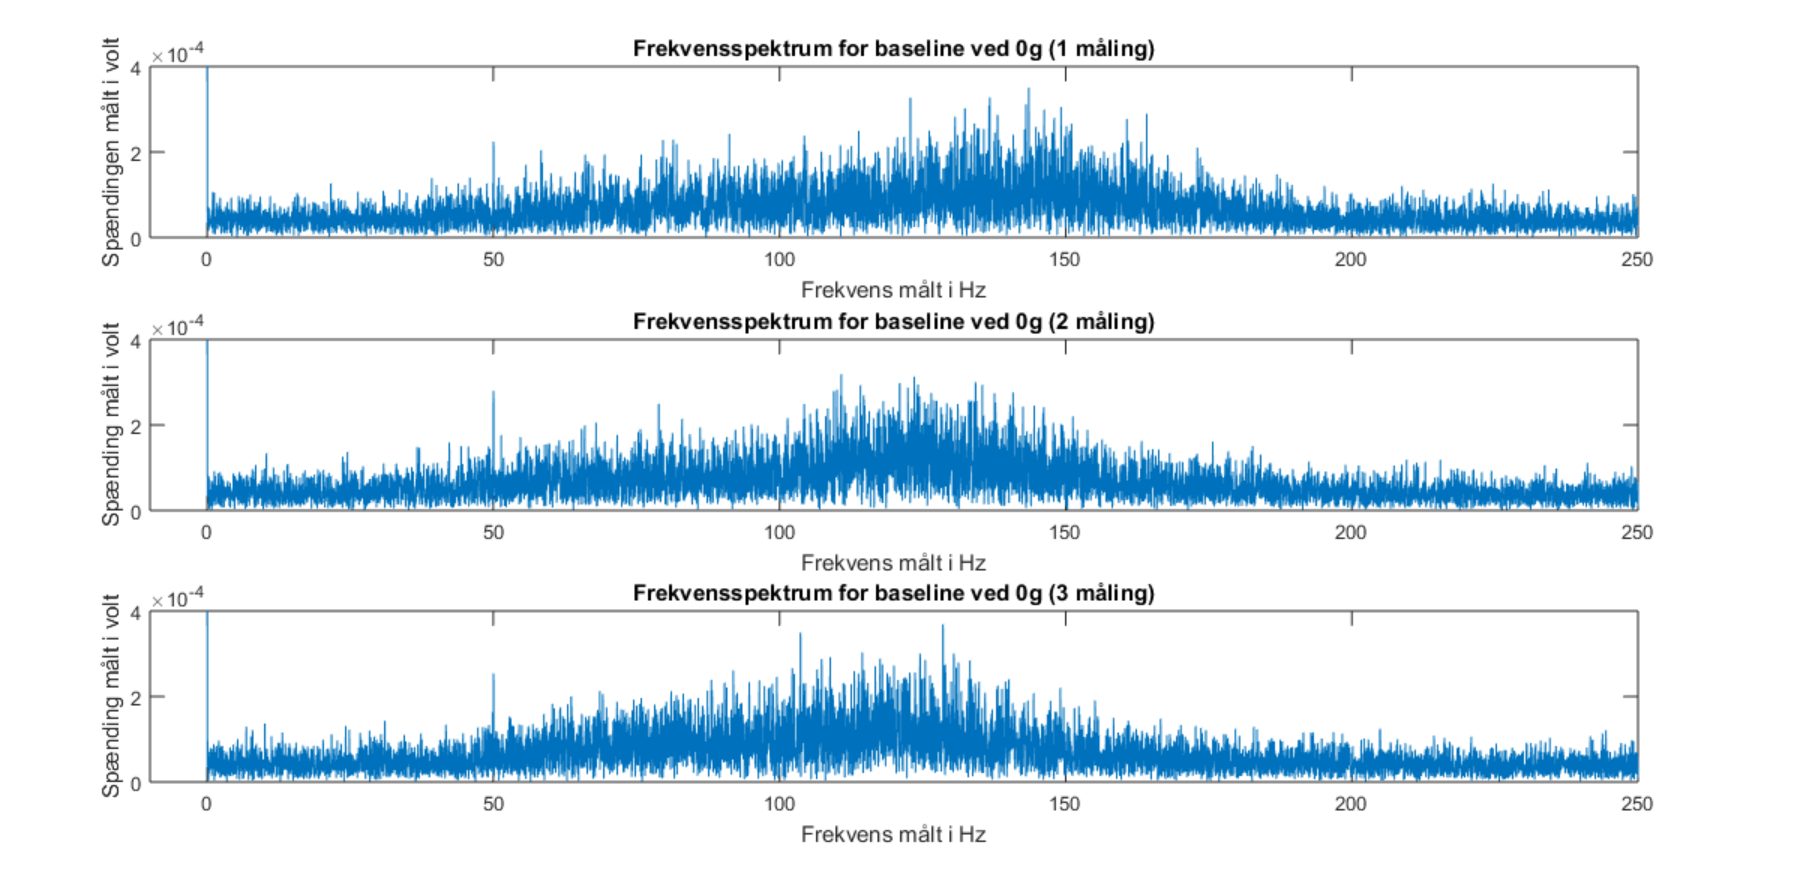
\includegraphics[scale=0.5]{figures/cProblemloesning/Pilotforsoeg_Frekvens0.png}
	\caption{På de tre grafer ses en FFT af første, anden og tredje måling ved en $0g$ påvirkning af accelerometret. Peaken ved $0Hz$ går op til ca. $1.58V$, men dette ses ikke på grafen, da resten af værdierne derved vil være meget svære at se.}
	\label{Fig:Pilot_FFT0}
\end{figure}
\begin{figure}[H]
	\centering
	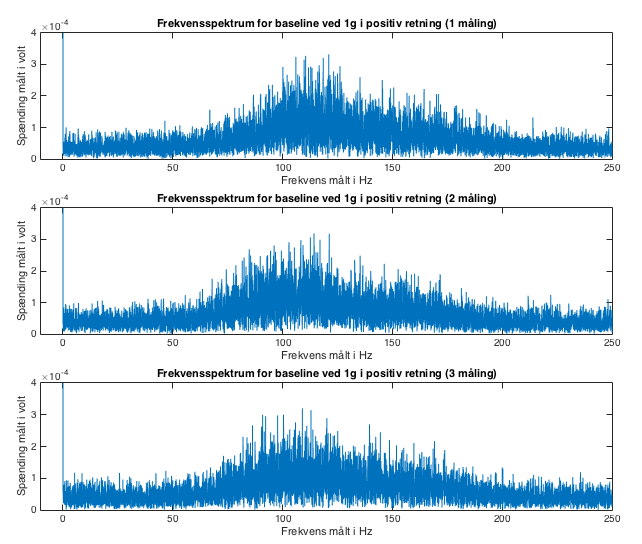
\includegraphics[scale=0.5]{figures/cProblemloesning/Pilotforsoeg_FrekvensP.png}
	\caption{På de tre grafer ses en FFT af første, anden og tredje måling ved en $1g$ påvirkning af accelerometret i positiv retning. Peaken ved $0Hz$ går op til ca. $1.86V$, men dette ses ikke på grafen, da resten af værdierne derved vil være meget svære at se.}
	\label{Fig:Pilot_FFTP}
\end{figure}
\begin{figure}[H]
	\centering
	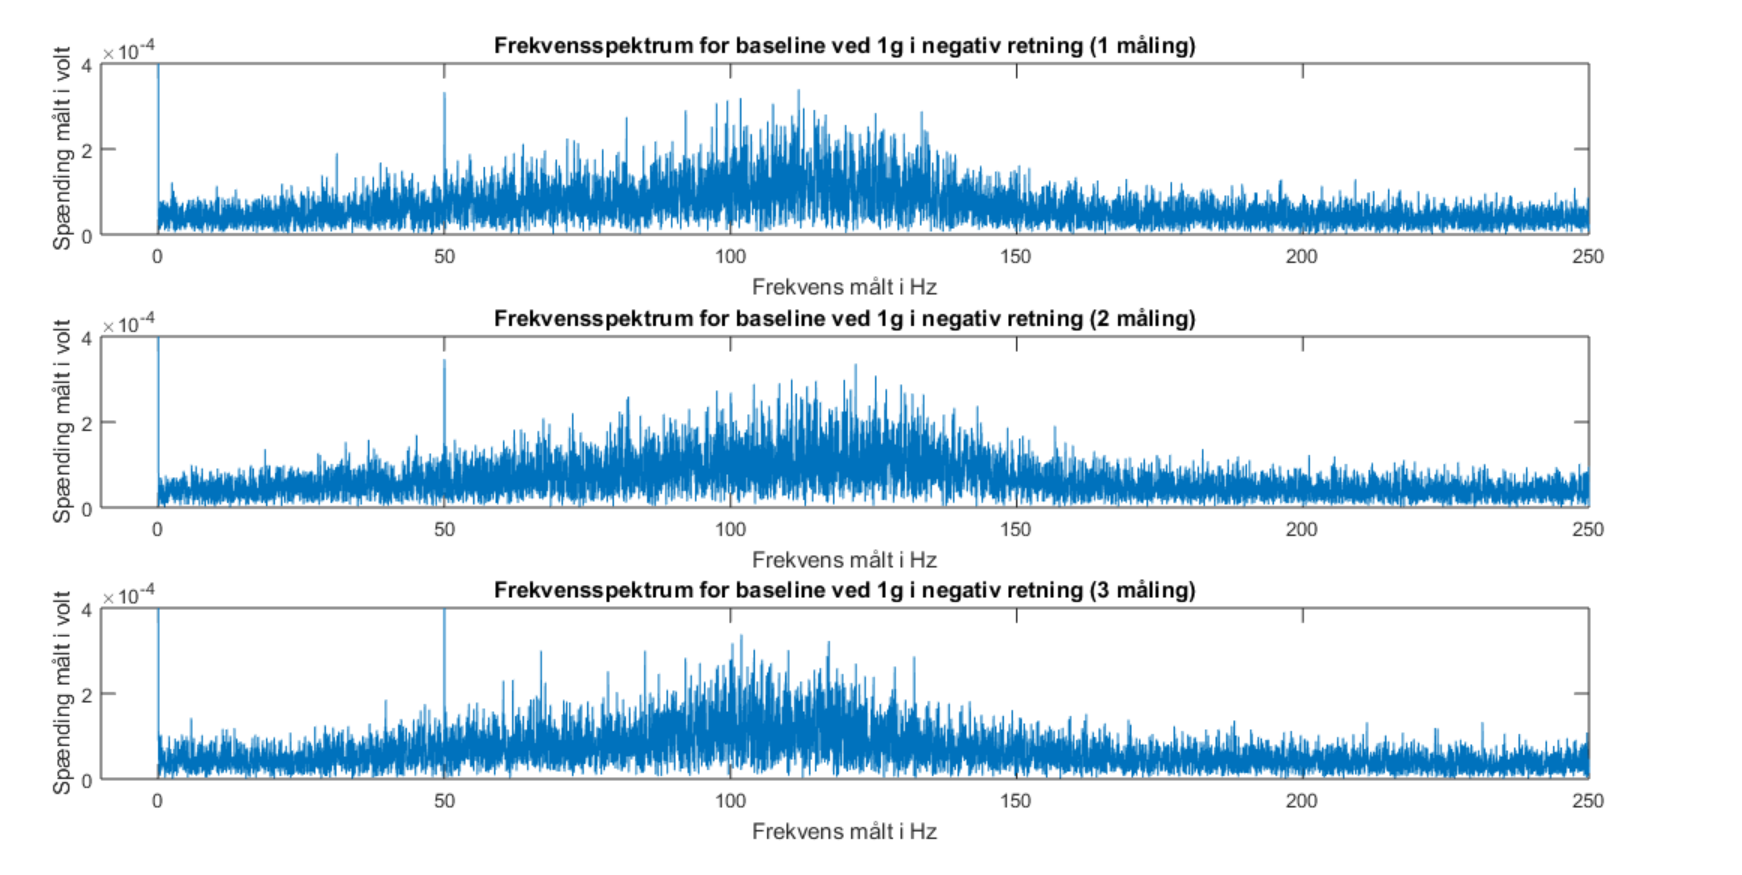
\includegraphics[scale=0.5]{figures/cProblemloesning/Pilotforsoeg_FrekvensN.png}
	\caption{På de tre grafer ses en FFT af første, anden og tredje måling ved en $1g$ påvirkning af accelerometret i negativ retning. Peaken ved $0Hz$ går op til knap $1.33V$, men dette ses ikke på grafen, da resten af værdierne derved vil være meget svære at se.}
	\label{Fig:Pilot_FFTN}
\end{figure}

\noindent Der ses på graferne, at signal to noise ratioen er lav, hvilket betyder, at der ikke er meget støj ift. ønsket signal. Der ses altså, at accelerometerets frekvensområde ligger i de lave frekvenser. Der ses ved en statisk acceleration at, signalet stort set kun er til stede ved $0Hz$. Alt over $0Hz$ betragtes derfor som støj. 

\begin{figure}[H]
	\centering
	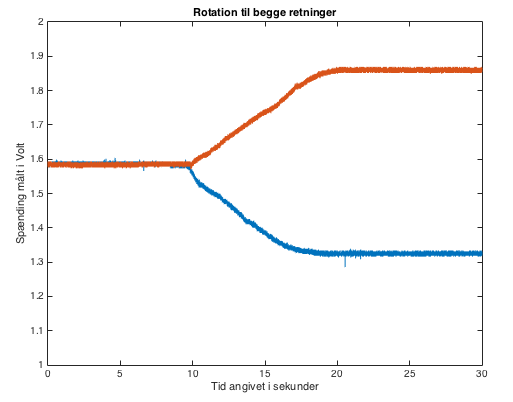
\includegraphics[scale=0.45]{figures/cProblemloesning/Pilotforsoeg_Rotation.png}
	\caption{På graferne ses accelerometerets output ved rotation fra $0g$ påvirkning til $1g$ påvirkning. Den orange graf repræsenterer rotation i positiv retning, hvorimod den blå graf repræsenterer rotation i negativ retning.}
	\label{Fig:Pilot_Rottid}
\end{figure}
\begin{figure}[H]
	\centering
	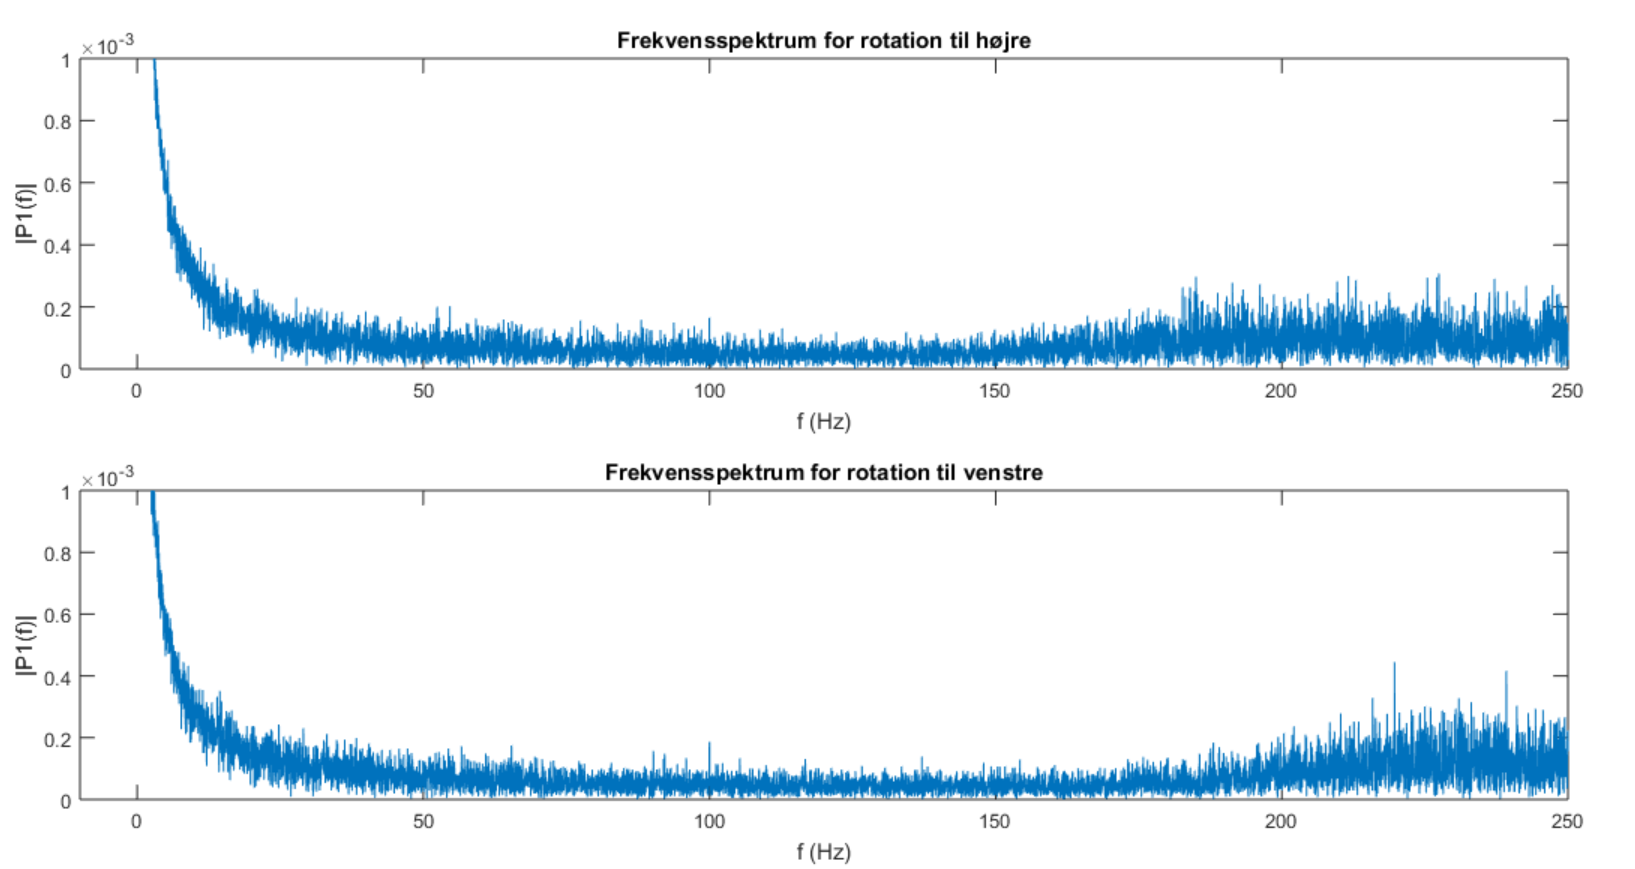
\includegraphics[scale=0.5]{figures/cProblemloesning/Pilotforsoeg_RotationFrekvens.png}
	\caption{På graferne ses en FFT af målinger for rotation i henholdsvis positiv og negativ retning.}
	\label{Fig:Pilot_Rotfrek}
\end{figure}
På \figref{Fig:Pilot_Rottid} ses der en lineær sammenhæng imellem g-påvirkning af accelerometret og outputtet. Der ses, at de tre baselines ved $0g$ påvirkning samt $1$g påvirkning i henholdsvis positiv og negativ retning, som måles i de første og sidste $10$ sekunder af målingen, stemmer overens med de målte baselines uden rotation. \\
På \figref{Fig:Pilot_Rotfrek} ses en FFT af målingerne af rotationerne. Ud fra dette kan der ses, at der er kommet større udsving i de lavere frekvenser fra $0-$ til ca. $25Hz$ sammenlignet med de statiske baseline målinger. Signalet regnes altså for at være i frekvensspektrummet $0-25Hz$. Alt uden for dette spektrum regnes derfor som støj.

\subsection{Diskussion og konklusion}
Der kan argumenteres for og imod at accelerometret er blevet udsat for $0g$ påvirkning, da det kan være svært at vurdere hvorvidt bordet er plant. Bordets hældning blev målt med et vaterpas, men der er mulighed for, at vaterpasset kan være upræcist. Accelerometret har desuden ujævnheder på overfladen i form af ledninger, hvilket kan betyde, at det muligvis ikke har lagt plant på bordet. \\
Der kan også være faktorer som har betydning for $1g$ påvirkningen, da vinklen nødvendigvis ikke er helt vinkelret. Ujævnheder på accelerometret samt vores holdemåde på det kan også have påvirket målingen. \\
Accelerometerets output afhænger også af rumtemperaturen, da denne påvirker aksernes offset samt sensitiviteten. Ved dette forsøg var temperaturen før, under og efter forsøget X, X og X, hvilket vil gå ind og påvirke målingerne. \\
Alle disse faktorer som er udregnet for pilotforsøget kan have indflydelse på de afvigelser der fås ift. databladet for accelerometeret. Det er altså igennem forsøget lykkedes at udregne afvigelserne for offset samt sensitiviteten, som står i accelerometrets datablad.  \\

I outputsignalet fra accelerometret ved den statiske acceleration udgør alt over $0Hz$ støj, hvorimod det vurderes, at alt over $25$Hz for rotationsmålingerne er støj. Maksimum og minimum outputsignalet fra accelerometret vil for langsom rotation eller svajning henholdsvis være $1.8627V$ og $1.3254V$, hvilket bliver til $0.2712V$ og $-0.2660V$ efter offsettet er blevet justeret. \\

%%%%  Kildeliste
\begingroup
	\raggedright
		\bibliographystyle{unsrtnat}
		\bibliography{kilder}
\endgroup

%%%% Bilag
\begin{appendices}
	% !TeX spellcheck = da_DK
\chapter{Nervefysiologi}\label{AppNerve}
Kroppens nervesysten kan inddeles i to dele; det centrale nervesystem (CNS) og det perifere nervesystem (PNS). CNS inderholder hjernen og rygraden, mens PNS indebærer kommunikationen imellem CNS og kroppens øvrige dele. PNS kan yderligere opdeles i det somatiske nervesystem, som består af det motoriske og sensoriske nervesystem, og autonome nervesystem, som består af en sympatisk og parasympatisk del. Det somatiske nervesystem styrer kroppens bevidste bevægelser og sender afferente signaler tilbage til CNS, hvorimod det autonome nervesystem regulerer kroppens ubevidste funktioner. Det er altså PNS, som registrerer signaler, CNS integrerer disse signaler og dirigerer et motorisk signal, som PNS skal omsætte til en handling. \cite{Martini2012,Stanfield2014} Et overblik over alt dette ses på \figref{Nersys}.

\begin{figure}[H]
	\centering
	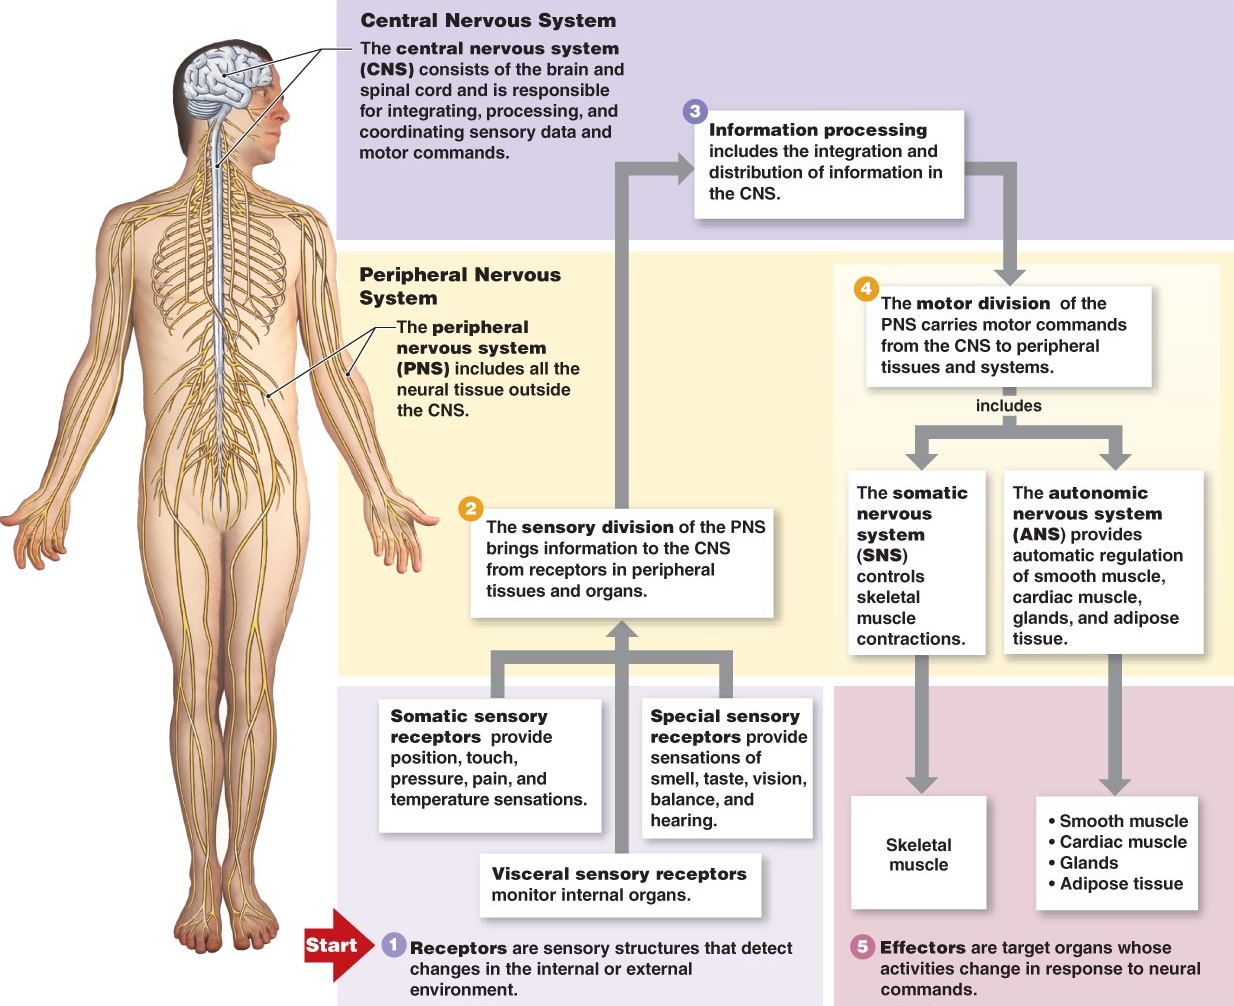
\includegraphics[scale=0.8]{figures/bProblemanalyse/Nervesys.jpg}
	\caption{Her ses et flowdiagram over, hvad der sker, når kroppen modtager et signal og skal processere dette om til en handling. Der ses desuden også en inddeling af CNS pg PNS med dets underdelinger. \cite{2015}}
	\label{Nersys}
\end{figure}

\section{Hjernens anatomi}
Cerebrum er encephalons største del og er involveret i sanseintegration, styring af frivillige bevægelser og højere intellektuelle funktioner, såsom tale og abstrakt tænkning. \cite{Academic2015b} Cerebrums ydre lag hedder cerebral cortex men kaldes hjernens grå substans. Her ligger nervers soma med dendritter. Cerebral cortex har forskellige centre, men kan også inddeles i højre og venstre halvdel. Delen af cerebral cortex der kontrollerer kroppens motorik med motor cortex kaldes gyrus præcentralis. Nerverne i dette område leder motoriske impulser til kroppens muskler igennem nervebanerne i den hvide substans, som indeholder nervernes axoner og fungerer derved som transportvej. \cite{Academic2015b,Martini2012,Stanfield2014} Disse axoner krydses i medulla oblongata og medulla spinalis og løber derefter til det modsatte legemeshalvdel fra, hvor impulsen afsendes. \cite{Martini2012}

	% !TeX spellcheck = da_DK
\chapter{Kroppens balance}\label{app-Balance}
%Apopleksipatienter oplever ofte problemer med balancen, da den ofte er nedsat eller slet ikke funktionsdygtig af forskellige årsager. \cite{Karnath2003} 
Proprioceptorer og sansereceptorer hjælper kroppen med balancen. Proprioceptorerne kontrollerer muskler, sener og leddenes position, hvorimod sansereceptorer er en bestemt slags celler, som f.eks. er placeret i ørerne og øjnene. \cite{Martini2012} Disse celler sender balanceinformationer til CNS og encephalon. Sansereceptorerne opfanger indtryk fra sanserne, som omsættes til bestemte signaler, der sendes til områder i cerebral cortex, cerebellum og centre i hele hjernestammen. Her bearbejdes informationen, hvorefter den korrekte fysiske position af kroppen og dens lemmer konkluderes. Når encephalon har bearbejdet indtrykkene, udsender den nerveimpulser til skeletmuskulaturen om at foretage jævne og koordinerede bevægelser, hvorved kropsbalancen opretholdes.\cite{Martini2012}

Øjet opfanger lys og er med til orienteringen af kroppen og dens lemmer. Hårceller i øret registrerer f.eks. hovedets bevægelser vha. tyngdekraften. Selvom et balanceorgan er ude af funktion, er kroppen stadig i stand til at opretholde balancen ved hjælp fra andre balanceorganer. Det er til gengæld vanskeligt for kroppen at opretholde balancen, hvis de behandlende centre i encephalon bliver skadet, som det kan ske ved apopleksipatienter. \cite{Martini2012} \\

\section{Ørets bidrag til balancen}
Øret består overordnet af tre dele; det ydre øre, mellemøret og det indre øre, som kan ses på \figref{Oeret}. 
\begin{figure}[H]
	\centering
	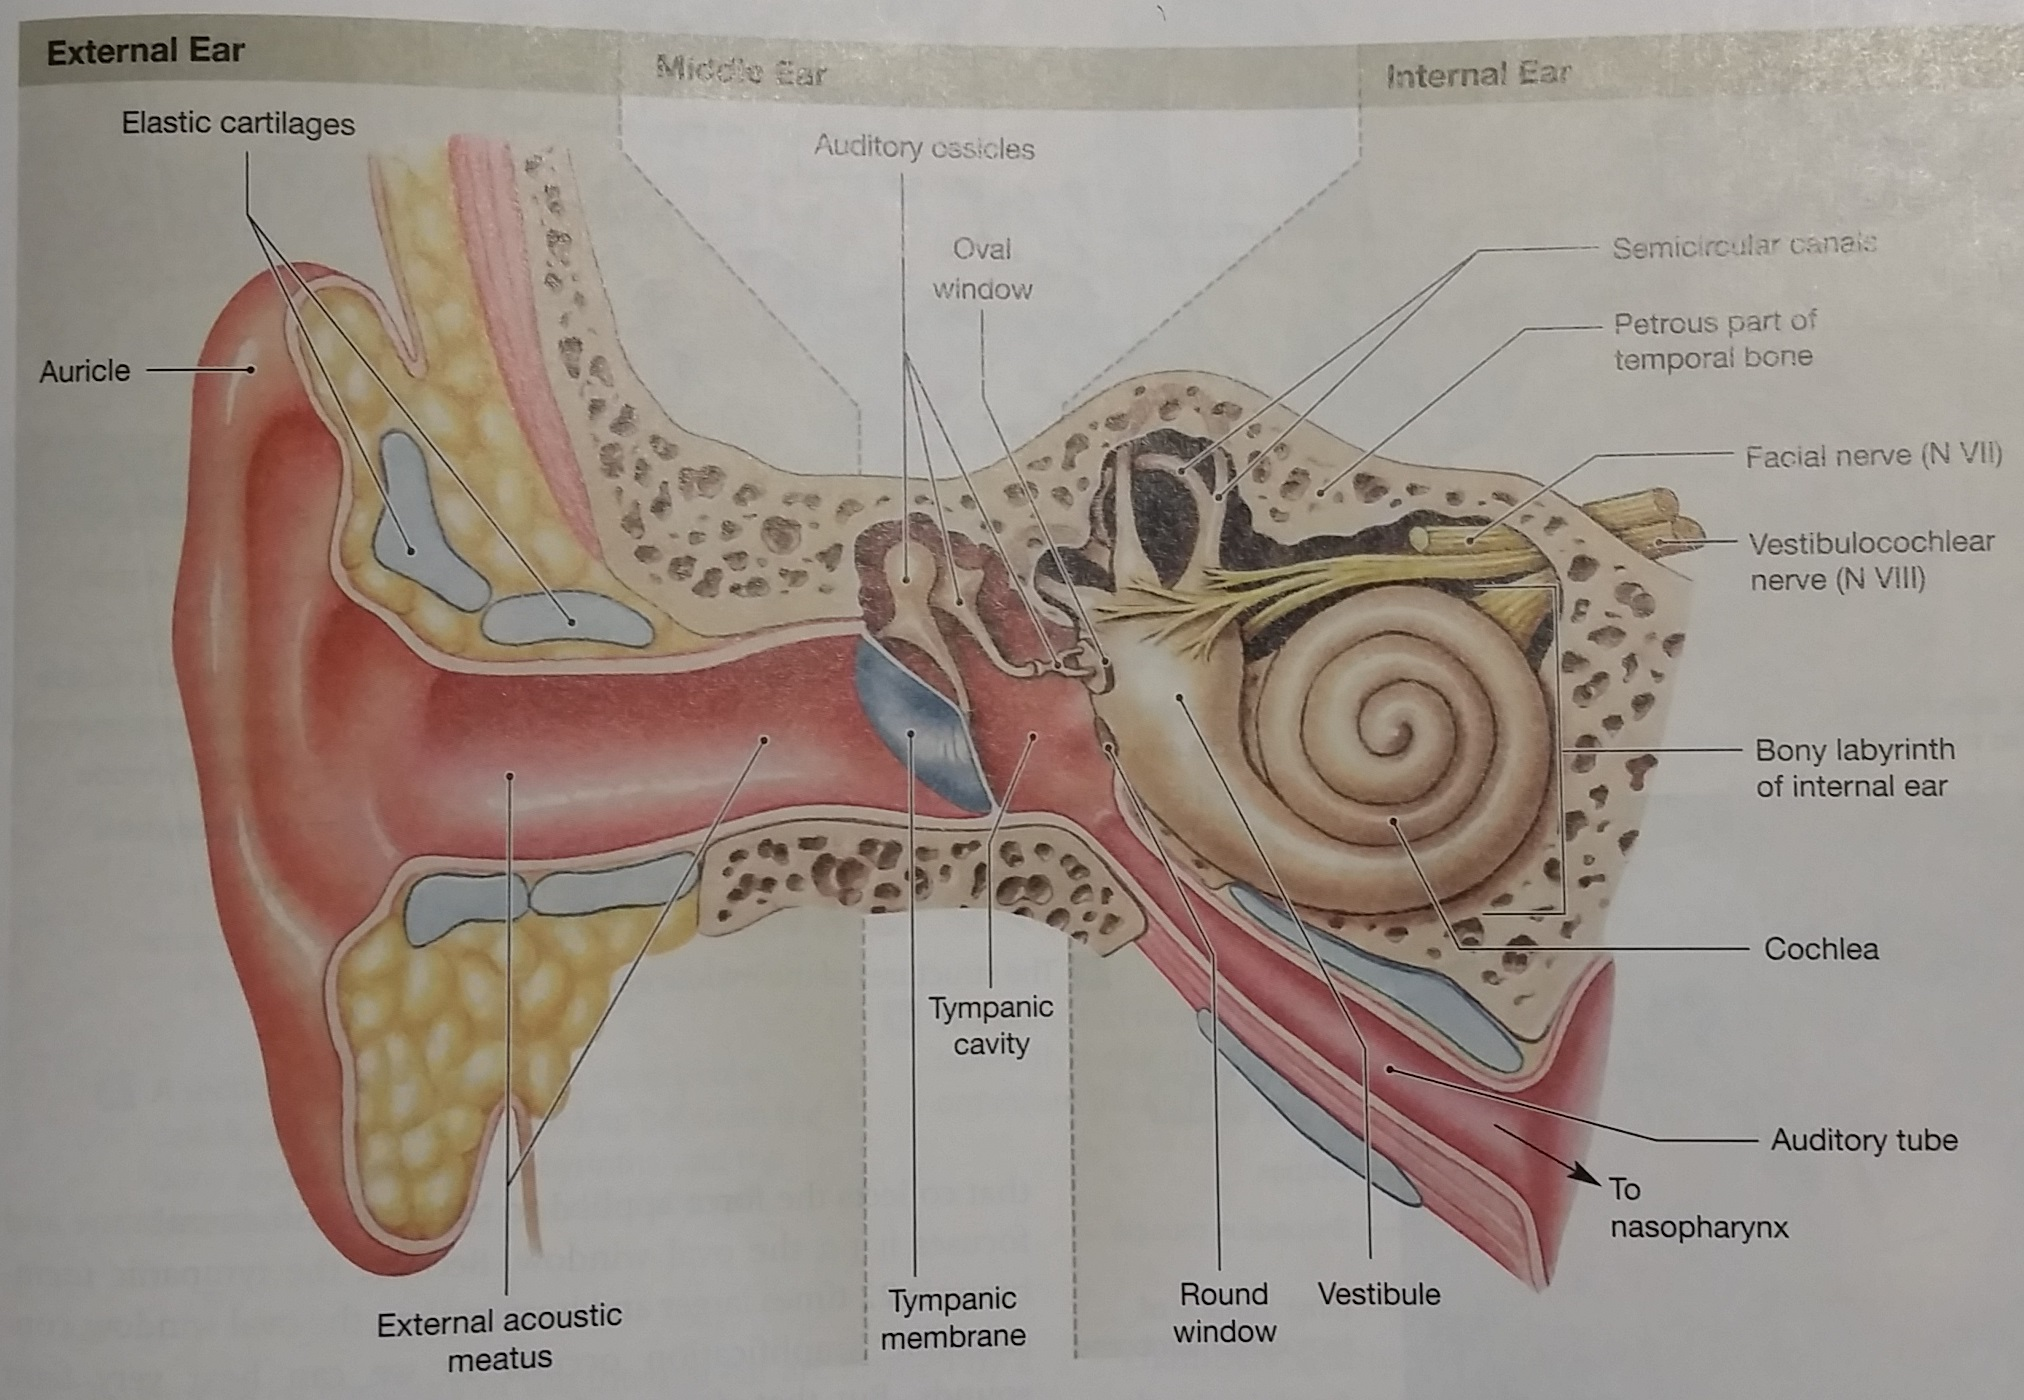
\includegraphics[scale=0.75]{figures/bProblemanalyse/Oerets-anatomi.jpg}
	\caption{På figuren ses ørets anatomiske opbygning \cite{Martini2012}.}
	\label{Oeret}
\end{figure}
Det indre øre er med til at kontrollere balancen vha. hårcellerne, som sættes i bevægelse. Det ydre øre modtager trykbølger, som sætter trommehinden i svingninger. Disse transporteres af mellemørets knogler, der forstærker svingningerne. Væsken i mellemøret modtager svingningerne fra knoglerne, hvilket sætter væsken i bevægelse. Denne bevægelse trækker i hårcellerne, og der skabes derved et aktionspotentiale. I det indre øre findes et netværk af sammenhængende væskeholdige kanaler, som er indkapslet i knoglen. Det er i disse kanaler receptorerne sidder. Det indre øre kan opdeles i tre undergrupper; vestibulen, øresneglen og buegangen. De centrale dele, der er relateret til balancen, er vestibulen og buegangen, hvorimod øresneglen kun bidrager til hørelsen. \cite{Martini2012}

Vestibulen består af to membransække; sacculen og utriclen, der opfanger sanseindtryk vedrørende tyngdekraft og lineær acceleration. Buegangens sansereceptorer opfanger stimuli omkring hovedets bevægelse, og hvor hurtigt bevægelsen foregår. Sansereceptorerne er placeret i buegangens tre væskefyldte knoglekanaler ved ampulla, der er forbundet til utriclen. Hårcellerne er kun aktive, når kroppen er i bevægelse ved at videregive information vedrørende hovedets bevægelse ift. tyngdekraften. Når hovedet er i bevægelse, sættes væsken i kanalerne også i bevægelse således, at væskebevægelser i den ene retning stimulerer hårcellerne, mens bevægelser i den modsatte retning forhindrer dem. For at få mest mulig information angående hovedets position, stimuleres de tre buegange af forskellige hovedbevægelser. Bevægelsesinformationerne sendes via vestibulocochlearnerven, der sender både information vedrørende balancen og hørelsen til encephalon i området mellem pons og medulla oblongata. \cite{Martini2012}    

\section{Øjets bidrag til balancen}
Synet er en central faktor for, hvordan encephalon holdes informeret omkring kroppens balance og generelle orientering. Dette gøres ved at give et indtryk af, hvordan kroppen og dens lemmer er placeret ift. omgivelserne. \cite{Schulmann1987} Øjet har tre hinder; fibrøs hinde, uvea og retina, som kan ses på \figref{Oejet}.
\begin{figure}[H]
	\centering
	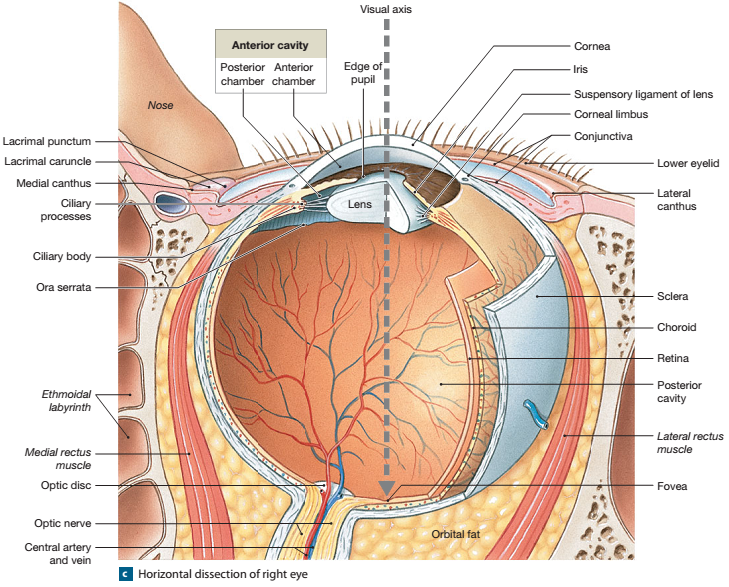
\includegraphics[scale=0.75]{figures/bProblemanalyse/Oejets-anatomi.png}
	\caption{På figuren ses øjets anatomisk opbygning. \cite{Martini2012}}
	\label{Oejet}
\end{figure}
Den fibrøse hinde\fxnote{NTK: hornhinden} er den yderste, som beskytter og støtter øjet. Den midterste hinde, kaldet uvea, indeholder blod og lymfekar samt regulerer mængden af lys, der kommer ind i øjet. Retina\fxnote{NTK: nethinden} er den inderste hinde, som er placeret bagerst i øjet. Den består af en pigmentdel og en indre neuraldel. Den neurale del indeholder fotoreceptorer, bestående af stave og tappe. Stave er følsomme overfor skarpt lys og gør det muligt at se i mørke. Tappe er følsomme overfor farvers bølgelængde, hvilket giver farvesyn. Pigmentdelen absorberer lys, der passerer gennem den neurale del og gør, at lyset ikke har mulighed for at reflektere tilbage. Foto- og lysreceptorerne konverterer lyset fra omgivelserne til elektrisk nervesignal, der giver information omkring det objekt, der betragtes, herunder dets størrelse, form og bevægelser. Informationerne processeres således, at horisontale celler lokaliserer områdets størrelse. Hvis der er kommet tilstrækkeligt med lys ind, sendes informationen først til bipolære celler herefter via synsnerven til det visuelle cortex, hvor informationen bearbejdes. \cite{Martini2012}     

\section{Proprioceptorerne og skeletmuskulaturens bidrag til balancen}
Proprioceptorer monitorerer leddenes position, muskelkontraktioners tilstand, samt spændingen i ledbånd og sener. Disse er placeret i skeletmuskulaturen. Informationerne sendes via nervesignaler til medulla spinalis og herfra igennem CNS til cerebellum. Proprioceptorer inddeles i tre overordnet grupper; muskelspindlere, golgi-sene organer og receptorer i ledkapsler. \cite{Martini2012}

Muskelspindlere styrer og kontrollerer ændringer af muskellængder og kan udløse en strækrefleks. Den sensoriske nerve er forbundet centralt på muskelspindleren, hvor den kontinuert sender sensoriske impulser til CNS. Hvis den sensoriske nerve modtager stimuli, i form af stræk, vil den motoriske nerve på muskelspindleren blive stimuleret. Stimulation af den motoriske nerve vil forkorte musklens længde. Nogle strækreflekser er holdningsreflekser, som hjælper til at holde balancen. I stående position kræves der et samarbejde mellem forskellige muskelgrupper for at forblive stående. Dette ses f.eks. hvis kroppen lænes forover, vil strækreflekserne i læggene blive aktiveret og kontraherer. Derved vil kroppen læne sig bagud og igen stå i en opret position. Hvis der sker en overkompensation fra lægmusklerne og kroppen læner sig for meget bagud, vil strækreflekser i skinnebenet og lårene aktiveres. Derved vil kroppen læne sig forover igen. Kroppen foretager mange af disse ubevidste korrektioner. \cite{Martini2012}   %(Se Martini 9th side 438 under "monosynaptic reflexes")

Golgi-sene organer sidder i en kløft\fxnote{NTK: kaldes junction på engelsk} mellem skeletmusklen og tilhørende sene. Dendritterne fra golgi-sene organet kobler sig på den nærmeste sene og stimuleres af spændingen i denne, hvorved den eksterne spænding i en muskelkontraktion bliver målt. \cite{Martini2012} 

Ledkapsler er fyldt med frie nerveender, som kaldes receptorer. Disse receptorer detekterer tryk, spænding og bevægelse i leddet. \cite{Martini2012}    \\
Det er en lille del, af den information proprioceptererne sender, der opfanges af bevidstheden, eftersom størstedelen foregår på et underbevidst niveau. \cite{Martini2012} \\


%Golgi seneorganer (Se Martini 9th side 501 under 15-3 propriocetor) %Receptorer i ledkapsler (Se Martini 9th side 501 under 15-3 propriocetor)

%\subsection{Apopleksi og balance}
%Balancen er styrer flere steder i kroppen og er med til at beskytte kroppen mod f.eks. faldulykker, ved at sikre at kroppen og den lemmer bevæger sig i kontrollerede og jævne bevægelser. Kroppen opretholder balancen ved at bruge ørerne, øjne og proprioceptorer i skeletmuskulaturen. Proprioceptorerne kontrollerer muskler, sener og leds position. Øjne opfanger lys og er med til orienteringen af kroppen og dens lemmer og hårceller i øret register hoveds bevægelser ved hjælp af tyngdekraften. Selvom et balanceorgan er ude af funktion er kroppen stadig i stand til at opretholde balancen ved hjælp fra andre balanceorganer. Det er til gengæld svære for kroppen at opretholde balancen hvis centrene i hjerne, som behandler den information, som kommer fra balanceorganerne, bliver skadet, som det kan ske ved apopleksi patienter. \cite{Martini2012}
% [1] – Martini, Frederic H and others. Fundamentals of Anatomy & Physiology (Kapitel:13, 14, 15, 17 ). 2012. Pearson. 
% [2] - Karnath2003
\end{appendices}

\end{document}